\renewcommand{\theequation}{\thesection.\arabic{equation}}
\renewcommand{\thetable}{\thesection.\arabic{table}}
\renewcommand{\thealgorithm}{\thesection.\arabic{algorithm}}
\renewcommand{\thefigure}{\thesection.\arabic{figure}}
\section{Whittle's Index }\label{app:whittle}
Whittle's index is computed for each agent. 
At each time $t$, given $\bm s_t$, the top $B$ agents with the highest indices are selected.
Whittle's index policy has two variants, each aimed at maximizing a different objective in an \emph{infinite} horizon setting: one for maximizing average reward and the other for maximizing discounted reward.
% Whittle's index policy has two variants based on the objective it is trying to maximize in an \emph{infinite} horizon. To be specific, Whittle's index policy has been defined for maximizing average reward and discounted reward separately. 

\textbf{Average Reward:} In this case, Whittle's index policy is designed to approximately find the policy $\bm{\pi}_d$ that maximizes the average reward,
\begin{align}
    \max_{\bm{\pi}_d}~&\liminf_{T\to\infty}\frac{1}{TM}\E\left[\sum_{m=1}^M\sum_{t=0}^TR^m\left(s_t^m\right)\mid\bm{s}_0
    % \mid \bm{s}_0=(0,0,\cdots,0)
    \right]\notag\\
    \text{s.t.~}&\sum_{m=1}^M a_t^m\leq B,\forall t\in[T]\label{eq:optimization-average-reward}.
\end{align}
We will denote $J^*$ to be the optimal value of Problem \ref{eq:optimization-average-reward}. Instead of directly solving Problem \ref{eq:optimization-average-reward}, Whittle deals with the Lagrangian relaxation of Problem \ref{eq:optimization-average-reward}, which is stated in Problem \ref{eq:optimization-average-reward-relaxation}
\begin{equation}
    \max_{\bm{\pi}_d}~\liminf_{T\to\infty}\frac{1}{TM}\E\left[\sum_{m=1}^M\sum_{t=0}^TR^m\left(s_t^m\right)+\lambda\left(1-a_{t+1}^m\right)\mid\bm{s}_0
    % \mid \bm{s}_0=(0,0,\cdots,0)
    \right].\label{eq:optimization-average-reward-relaxation}
\end{equation}
The key observation to derive Whittle's index policy is that Problem \ref{eq:optimization-average-reward-relaxation} can be solved by addressing the following dynamic programming separately for each agent
\begin{align*}
    V^m_\lambda(s)&=\max_{a\in\{0,1\}} Q^m(s,a)\\
    Q^m_\lambda(s,a)+\beta^*_m&=R^m(s)-\lambda\mathbbm{1}\{a=1\}\\&+\sum_{s'\in\mathcal{S}}P^m_a(s,s')V^m(s'),
\end{align*}
where $\beta^*_m$ is the maximized average reward for arm $m$ without any constraint, i.e.
\begin{equation*}
    \beta^*_m:=\max~ \liminf_{T\to\infty}\frac{1}{T}\E\left[\sum_{t=0}^TR^m\left(s_t^m\right)\mid s_0^m
    % \mid \bm{s}_0=(0,0,\cdots,0)
    \right].
\end{equation*}
The Whittle's index $\lambda^m_s$ is defined as the multiplier $\lambda_s^m$ when it is equally favorable between choosing action $1$ and action $0$, i.e. $Q^m_{\lambda^m_s}(s,1)=Q^m_{\lambda^m_s}(s,0)$. The Whittle's index policy would then give action to $B$ agents with the highest Whittle's index at each time step $t$. Denote this as $\bm{\pi}^{\text{Whittle}}$ and the average reward of Whittle's index policy as $J^{\text{Whittle}}$. The performance of Whittle's index policy is characterized in Theorem \ref{th:optimality-whittle}.
\begin{theorem}[Theorem 2, \citealt{Weber_Weiss_1990}]\label{th:optimality-whittle}
Suppose all arms are homogeneous, i.e., $P_a^m=P_a^{m'}, R^m=R^{m'},\forall m\neq m'$, then the Whittle's index policy is asymptotically optimal,
\begin{equation*}
    \lim_{M\to\infty}J^{\text{Whittle}}=\lim_{M\to\infty}J^*.
\end{equation*}
\end{theorem}

\textbf{Discounted Reward:} In this case, Whittle's index policy is designed to approximately find the policy $\bm{\pi}_d$ that maximizes the discounted reward for a fixed discount factor $\beta$,
\begin{align}
    \max_{\bm{\pi}_d}~&\sum_{t=0}^{\infty}\frac{1}{M}\E\left[\sum_{m=1}^M\beta^tR^m\left(s_t^m\right)\mid\bm{s}_0
    % \mid \bm{s}_0=(0,0,\cdots,0)
    \right]\notag\\
    \text{s.t.~}&\sum_{m=1}^M a_t^m\leq B,\forall t\in[T]\label{eq:optimization-discounted-reward}.
\end{align}
Similarly, instead of directly solving Problem \ref{eq:optimization-discounted-reward}, Whittle deals with the Lagrangian relaxation of Problem \ref{eq:optimization-discounted-reward}, which is stated in Problem \ref{eq:optimization-discounted-reward-relaxation}
\begin{equation}
    \max_{\bm{\pi}_d}~\sum_{t=0}^{\infty}\frac{1}{M}\E\left[\sum_{m=1}^M\beta^t\left(R^m\left(s_t^m\right)+\lambda\left(1-a_{t+1}^m\right)\right)\mid\bm{s}_0
    % \mid \bm{s}_0=(0,0,\cdots,0)
    \right].\label{eq:optimization-discounted-reward-relaxation}
\end{equation}
Again, the same key observation is that Problem \ref{eq:optimization-discounted-reward-relaxation} can be solved by addressing the following dynamic programming separately for each agent
\begin{align}
    V^m_\lambda(s)&=\max_{a\in\{0,1\}} Q^m(s,a)\notag\\
    Q^m_\lambda(s,a)&=R^m(s)-\lambda\mathbbm{1}\{a=1\}\notag\\&+\beta\sum_{s'\in\mathcal{S}}P^m_a(s,s')V^m(s').\label{eq:dynamic-programming-discounted}
\end{align}
The definition of Whittle's index will be the same in the average reward case.
% \kyra{add discounted Whittle's index}
\subsection{Generalized Regret in Online Restless Bandits}\label{app:generalized_regret}
Given $K$ episodes each with a horizon length of $T$ and the set of online Whittle's index policy at each episode $k\in[K]$, $\bm\omega:=\{\bm \omega_k\}_{k\in[K]}$, the regret $\mathcal{R}_{f}(\bm{\omega})$:
% To evaluate the performance of the online approximation of the Whittle's index policy, the notion of regret is defined, which is directly comparing with the finite-horizon performance of the Whittle index policy and average them among $K$ number of episodes.
\begin{align}\label{eq:regret-finite-horizon-general}
\mathcal{R}_{f}(\bm{\omega}):&=\frac{1}{K}\sum_{k=1}^K\Bigg(\E_{\bm{\pi}^{\text{Whittle}}}\left[\sum_{m=1}^M\sum_{t=0}^TR^m\left(s_t^m\right)\mid\bm{s}_0
    % \mid \bm{s}_0=(0,0,\cdots,0)
    \right]-\E_{\bm{\omega}_k}\left[\sum_{m=1}^M\sum_{t=0}^TR^m\left(s_t^m\right)\mid\bm{s}_0
    % \mid \bm{s}_0=(0,0,\cdots,0)
    \right]\Bigg).
\end{align}
We note that our problem setting corresponds to the scenario where $K=1$.

Existing regret bounds on online Whittle's index policy are only meaningful when the number of episodes is sufficiently large. 
% For regret bound of existing online Whittle's index policy, it will only be reasonable when the number of episodes is sufficiently large. 
To illustrate this, \citet{wang2023optimistic} shows that their algorithm has a regret bound of the order $\mathcal{O}\left(T\sqrt{TK}\right)$. If we only have $1$ episode, this will be equivalent to saying that the regret bound is $\mathcal{O}(T^{3/2})$. The hardness lies in estimating the MDP:  \citealt{azar2017minimax} show that when $B=M=1$, the lower bound of the regret is $\Omega(T\sqrt{K})$. This lower bound indicates that when directly dealing with an MDP, it is impossible to get a regret bound that is sublinear in $T$. 


% {\color{orange}{
% ivan: jm, if this notation is inconvenient, the feel free to ignore this block. I am going to continue verifying your proof using it here.
% %
% ivan: This is merely a suggestion, but you might want to consider the following notation to improve readability, use the vertical space more efficiently, and shorten the eqns (mostly those that feature derivations using explicit state-action indices):
% \begin{itemize}
%     \item instead of $s'$ (S-prime) we denote the next state as $x$ (or some other one-letter symbol);
%     \item since all our spaces (state and action) are finite why not use $q^m_{sax}$ to denote the $m$-th agent's probability of $s \to x$ transition under $a$ given by $P^m_a(s'=x \mid s)$;
%     \item simply use sub-scripted values for evaluations of functions, e.g. use $f_1$ for $f(1)$ for a function $f \colon S \to \mathbb{R}$.
% \end{itemize}
% For example, below is the corrected proof of lemma \ref{le:iff-for-dominance}.

% \begin{paragraph}{Proof of Lemma \ref{le:iff-for-dominance}}
% ``assumption \ref{asssumption:stochastic-dominance} holds iff $P(1 \mid s, 1) \geq P(1 \mid s, 0)$ for any $s \in \{0, 1\}$''

% For a monotonic non-decreasing $f \colon S \to \mathbb{R}$ and for any $s \in S$ ($S = \{0, 1\}$) we have the following:
% \begin{align*}
% \E_{x \sim P(x\mid s, 1)} f_x - \E_{x \sim P(x\mid s, 0)} f_x
% % \E_{x \sim q_{s1x}} f_x - \E_{x \sim q_{s0x}} f_x
%     &
%         = f_1 q_{s11} + f_0 q_{s10} - f_1 q_{s01} - f_0 q_{s00}
%     \\
%     &
%         = \left(q_{s10} - q_{s00} \pm 1\right) f_0 + \left(q_{s11} - q_{s01}\right) f_1
%         % = - \left(q_{s11} - q_{s01}\right) f_0 + \left(q_{s11} - q_{s01}\right) f_1
%         = \left(q_{s11} - q_{s01}\right) \left(f_1 - f_0\right)
%     \,,
% \end{align*}
% because $q_{sax}$ is the transition probability $P(s' = x \mid s, a)$, and $q_{sa0} + q_{sa1} = 1$. Since $f_0 \leq f_1$, the sign of left-hand side is completely determined by the difference $q_{s11} - q_{s01}$ in the right-hand side. Therefore, $\E_{x \sim q_{s1x}} f_x \geq \E_{x \sim q_{s0x}} f_x$ if and only if $q_{s11} \geq q_{s01}$ for all $s \in S$. QED
% \end{paragraph}

% \begin{paragraph}{Proof of Lemma \ref{le:optimality-one-agent}}  % finite horizon case
% ``if $r$ is monotonic, then under \ref{asssumption:stochastic-dominance} action $1$ is optimal''
% % ivan: TODO
% % hypothesis: abstract away the details by using monotonicy of $T_\ast$, that it is a contraction, and some VI argument
% \end{paragraph}
% }}

\section{Counter Example for Heterogeneous Agents}\label{sec:counter-example-heterogeneous}
In this section, we will construct an instance involving heterogeneous agents where the greedy policy is not optimal. Say that each agent is associated with two state: State 0 and State 1, and the agent can
take either Action $1$ (intervention) or Action $0$ (no intervention). Assume for now that there are \textbf{4} agents with different transition probabilities. 
The first two agents fall under Type 1:
% For the first two agents, 
% the
their transition probability under Action 1 is shown in Figure \ref{fig:transition-1-1} 
% when given intervention 
and their transition probability under Action 0
% without intervention
is shown in Figure \ref{fig:transition-1-0}. 
The other two agents fall under Type 2:
% Meanwhile, for the other two agents,
their transition probability under Action 1
% with intervention 
is shown in Figure \ref{fig:transition-2-1} and their transition probability under Action 0 
% without intervention
is shown in Figure \ref{fig:transition-2-0}. 
\begin{figure}[!h]
\centering
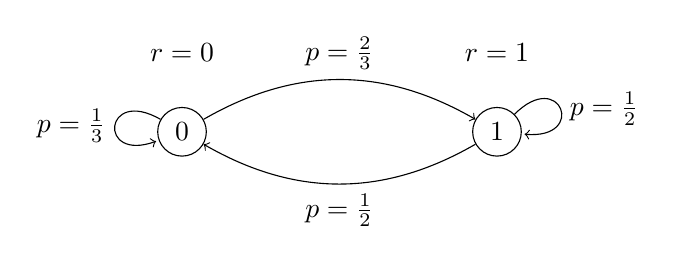
\begin{tikzpicture}
  % States
 \node[circle, draw] (0) at (0,0) {$0$};
  \node[circle, draw] (1) at (4,0) {$1$};
  
  % Arrows
  \draw[->] (0) edge[out=150, in=200, loop] node[left] {$p=\frac{1}{3}$}  (1);
  \draw[->] (1) edge[out=45, in=355, loop] node[right] {$p=\frac{1}{2}$}  (0);
  \draw[->] (0) to[bend left]  node[above] {$p=\frac{2}{3}$}(1);
  \draw[->] (1) to[bend left] node[below] {$p=\frac{1}{2}$}(0);
   \node at (0,1) {$r=0$};
  \node at (4,1) {$r=1$};
\end{tikzpicture}
\caption{Dynamic of Agent Type 1 with Intervention}
\label{fig:transition-1-1}
\end{figure}
\begin{figure}[!h]
\centering
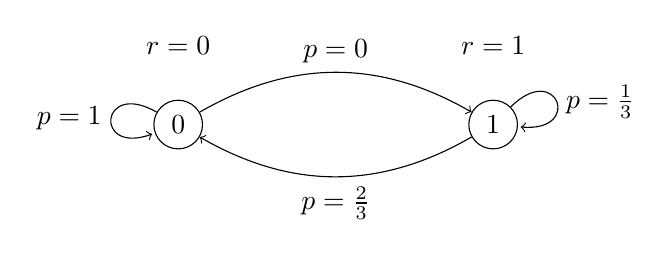
\begin{tikzpicture}
  % States
 \node[circle, draw] (0) at (0,0) {$0$};
  \node[circle, draw] (1) at (4,0) {$1$};
  
  % Arrows
  \draw[->] (0) edge[out=150, in=200, loop] node[left] {$p=1$}  (1);
  \draw[->] (1) edge[out=45, in=355, loop] node[right] {$p=\frac{1}{3}$}  (0);
  \draw[->] (0) to[bend left]  node[above] {$p=0$}(1);
  \draw[->] (1) to[bend left] node[below] {$p=\frac{2}{3}$}(0);
   \node at (0,1) {$r=0$};
  \node at (4,1) {$r=1$};
\end{tikzpicture}
\caption{Dynamic of Agent Type 1 without Intervention}
\label{fig:transition-1-0}
\end{figure}
\begin{figure}[!h]
\centering
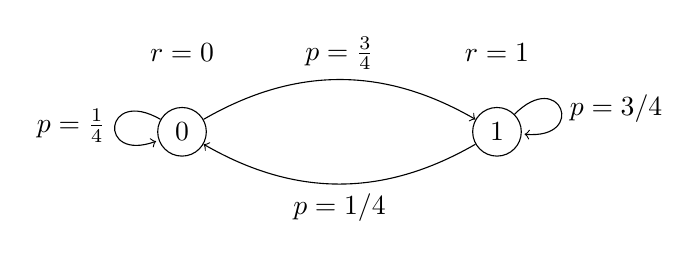
\begin{tikzpicture}
  % States
 \node[circle, draw] (0) at (0,0) {$0$};
  \node[circle, draw] (1) at (4,0) {$1$};
  
  % Arrows
  \draw[->] (0) edge[out=150, in=200, loop] node[left] {$p=\frac{1}{4}$}  (1);
  \draw[->] (1) edge[out=45, in=355, loop] node[right] {$p=3/4$}  (0);
  \draw[->] (0) to[bend left]  node[above] {$p=\frac{3}{4}$}(1);
  \draw[->] (1) to[bend left] node[below] {$p=1/4$}(0);
   \node at (0,1) {$r=0$};
  \node at (4,1) {$r=1$};
\end{tikzpicture}
\caption{Dynamic of Agent Type 2 with Intervention}
\label{fig:transition-2-1}
\end{figure}
\begin{figure}[!ht]
\centering
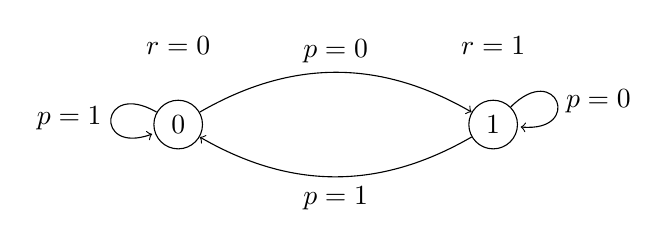
\begin{tikzpicture}
  % States
 \node[circle, draw] (0) at (0,0) {$0$};
  \node[circle, draw] (1) at (4,0) {$1$};
  
  % Arrows
  \draw[->] (0) edge[out=150, in=200, loop] node[left] {$p=1$}  (1);
  \draw[->] (1) edge[out=45, in=355, loop] node[right] {$p=0$}  (0);
  \draw[->] (0) to[bend left]  node[above] {$p=0$}(1);
  \draw[->] (1) to[bend left] node[below] {$p=1$}(0);
   \node at (0,1) {$r=0$};
  \node at (4,1) {$r=1$};
\end{tikzpicture}
\caption{Dynamic of Agent Type 2 without Intervention}
\label{fig:transition-2-0}
\end{figure}

Suppose the budget equals one, meaning that we can only give one agent intervention at each time. 
% In this example, 
We observe that under our problem setup Type 2 agents always have a higher incremental reward $\phi^2(1,1):=\frac{3}{4}\cdot 1, \phi^2(0,1):=\frac{3}{4}\cdot 1,\phi^2(s,0)=0,I^2(1)=I^2(0)=\frac{3}{4}$, opposed to $\phi^1(0,1)=\frac{2}{3}\cdot 1,\phi^1(1,1)=\frac{1}{2}\cdot 1,\phi^1(0,0)=0,\phi^1(1,0)=\frac{1}{3}, I(1)=\frac{2}{3},I(0)=\frac{1}{6}$. 
However, this does not imply that the optimal policy is to always take Action 1 for Type 2 agents. If all resources are allocated to Type 2 agents, the expected reward is $3/4$ per time step summed across all agents. Alternatively, if resources are devoted to Type 1 agents, alternating actions between the two Type 1 agents, the expected reward is $2/3 + 2/3 \times 1/3 = 8/9$ per Type 1 agent over two time periods (where an action is taken in one period but not in the other). To illustrate this point, we ran the following experiment:
we set the horizon to be $20$ and repeated the simulation $300$ times. We compare the performance of the following two policies in terms of cumulative rewards: Policy 1) choosing one of the Type 2 agents for intervention at each time, and Policy 2) alternating intervention between the two Type 1 agents. The observed cumulative for Policies 1 and 2 are 15.02 and 16.78, respectively. This shows that the greedy policy is not optimal under all heterogeneous agents cases even under Assumption \ref{asssumption:stochastic-dominance}.
\section{Technical Details In Section \ref{subsec:optimality}}\label{appendix:proof-of-reduction}
First, recall that
at each time $t$ of an offline restless bandit problem, 
the learner observes the set of states of $M$ agents, denoted by $\bm{s}_t:=\left(s_t^1,s_t^2,\cdots,s_t^M\right)$, and receives the corresponding reward $\bm{r}_t:=(r_t^1,\cdots, r_t^M)$. 
% Let $\boldsymbol{\mathcal{A}}$ denote the set of all possible action vectors, i.e.,  $\boldsymbol{\mathcal{A}}=\{0,1\}^M$.
Based on the observed states, the learner determines the action $\bm{a}_{t+1}:=\left(a_{t+1}^1,a_{t+1}^2,\cdots,a_{t+1}^M\right)$,  according to a deterministic policy $\pi^d_{t+1}(\bm{s}):\mathcal{S}^M\rightarrow 
\{0,1\}^M$.
% \kyra{add a sentence here talking about how the states transition to next time step.}
The learner is provided with a budget constraint, allowing at most $B$ arms to be pulled at each time step,
% the learner can pull at most $B$ arms,
i.e., $\sum_{m\in[M]} a_{t+1}^m\leq B$.
After pulling up to $B$ arms, the learner
% After choosing action $\bm{a}_{t+1}$, the learner can
observes the next state $\bm{s}_{t+1}$, 
% which is
generated according to $s_{t+1}^m\sim P_{a_{t+1}^m}^m\left(s_t^m,s_{t+1}^m\right)$, and 
% as well as
receives a feedback $\bm{r}_{t+1}$.

To ease notation, in Section \ref{appendix:proof-of-reduction} we will use $q^a_{ss'}(m)$ to denote $P_a^m(s,s')$.
Before presenting the proofs, we reformulate the online restless bandit problem as a single large MDP, where the state and action are defined as tuples comprising the composite states and actions of all agents. This reformulation is valid because the agents/arms in the restless bandit problem are independent. This MDP can be described as
% Before we introduce the technical details, we will first provide another approach to address the restless bandit and define some notations that will be used in the proof. Since we assume that each arms are independent, we can view this problem as a MDP itself with parameters 
$\left(\mathcal{S}^M,\mathcal{F},q,\bm{R}\right)$, where $\mathcal{F}$ is defined as
\begin{align*}
    \mathcal{F}:=\bigg\{&\left(a^1,a^2,\cdots,a^M\right):\left(a^1,a^2,\cdots,a^M\right)\in\mathcal{A}^M, \sum_{m=1}^M a^m\leq B\bigg\}.
\end{align*}
Let $q_{\bm s \bm s'}^{\bm a}:=\mathbb{P}(\bm s'|\bm s, \bm a) = P_{\bm a}(\bm s, \bm s')= \prod_{m=1}^M 
q^{a}_{ss'}(m)$, and let
%
% $q\left(\bm{s}'\mid\bm{s},\bm{a}\right)
% =\prod_{m=1}^M 
% q^{a^m}_{\left(s'\right), s}(m)$
% q^m\left(\left(s'\right)^m\mid s^m,a^m\right)$
% and 
$\bm{R}(\bm{s})=\sum_{m=1}^M r^m\left(s^m\right)$.
Then for each policy $\bm{\pi}$ and each time-step $h$, we can define the value function $V_h^{\bm{\pi}}(\bm{s})$ as
\begin{equation}\label{eq:value-function}
    \E_{\bm{\pi}}\left[\sum_{t=h}^T \bm{R}(\bm{s}_t)\mid \bm{s}_h=\bm{s}\right].
\end{equation}
With this definition, Problem \eqref{eq:optimization-problem} is equivalent to
\begin{equation*}
    \max_{\bm{\pi}} V_0^{\bm{\pi}}\left(\bm{s}_0\right).
\end{equation*}
Again, we use $\bm \pi^*:= \{\pi_{t}^*\}_{t\in[T]}$ to denote the maximizer, and let $V_h^*$ be the value function under policy $\bm \pi^*$. We will use this notation in Appendix~\ref{app:optimality-one-agent}, \ref{app:use-all-budget}, \ref{app:thm-optimality-greedy-homogeneous}, and \ref{app:proof-thresholding}.
% \kyra{note here in which subsections we will use this notation}


Next, we state the proofs.
% Now, we are ready to give the proofs.
\subsection{Proof of Lemma \ref{le:iff-for-dominance}}\label{app:stochastic-dominance}
\iffDominance*
\begin{proof}
% \kyra{this proof did not use the large MDP notation}
$\Rightarrow$:
    When Assumption \ref{asssumption:stochastic-dominance} holds, suppose
    % The proof proceeds by assuming that
    there exists $s\in\mathcal{S}$ such that $q_{s1}^1<q_{s1}^0$.
    % $q(1|s,1)<q(1|s,0)$.
    Without loss of generality (WLOG), assume $s=1$. We have for any increasing function $f$:
    \begin{align*}
        \E_{s'\sim q_{1s'}^1}\left[f(s')\right]-\E_{s'\sim q_{1s'}^0}\left[f(s')\right]
        &=f(1)q^1_{11}+f(0)q^1_{10}-f(1)q^0_{11}-f(0)q^0_{10}\\
        &=f(1)\left(q^1_{11}-q^0_{11}\right)+f(0)\left(q^1_{10}-q^0_{10}\right)\\
        &=\left(f(1)-f(0)\right)\left(q^1_{11}-q^0_{11}\right)\\
        &<0,
    \end{align*}
    where the last inequality holds because $f$ is increasing and the assumption that $q^1_{11}<q^0_{11}$. This will contradict Assumption \ref{asssumption:stochastic-dominance}. Therefore, we must have for all $s\in\mathcal{S}$, $q_{s1}^1\geq q_{s1}^0$.

$\Leftarrow:$  When for all $s\in\mathcal{S}$, $q_{s1}^1\geq q_{s1}^0$, we will prove Eq.~\eqref{eq:stochastic-dominance} separately for $s=0$ and $s=1$.
    % Suppose $q(1|s,1)\geq q(1|s,0)$,
   When $s=1$,  we have
     \begin{align*}
        \E_{s'\sim q_{1s'}^1}\left[f(s')\right]-\E_{s'\sim q_{1s'}^0}\left[f(s')\right]&=f(1)q^1_{11}+f(0)q^1_{10}-f(1)q^0_{11}-f(0)q^0_{10}\\
        &=f(1)\left(q^1_{11}-q^0_{11}\right)+f(0)\left(q^1_{10}-q^0_{10}\right)\\
        &=\left(f(1)-f(0)\right)\left(q^1_{11}-q^0_{11}\right)\\
        &\geq 0,
    \end{align*}
      where the last inequality holds because $f$ is increasing and the assumption that $q^1_{11}\geq q^0_{11}$. Similarly, we can show that $\E_{s'\sim q_{0s'}^1}\left[f(s')\right]\geq\E_{s'\sim q_{0s'}^0}\left[f(s')\right]$. This completes the proof.
\end{proof}
\subsection{Proof of Lemma \ref{le:optimality-one-agent}}\label{app:optimality-one-agent}
\optimalOneAgent*
\begin{proof}
We will use Bellman optimality equation to prove the theorem. Specifically, we only need to prove that for any $h$, the maximizer $a$ of the following problem,
\begin{equation*}
    V_h^{*}(s)=R(s)+\max_{a}\sum_{s'}q_{ss'}^aV_{h+1}^{*}(s),
\end{equation*}
aligns with $\pi_{h+1}^{\text{greedy}}(s)$. With Assumption \ref{asssumption:stochastic-dominance}, this is equivalent to showing $V_{h+1}^{*}(s)$ is an increasing function in $s$. To do this, we will discuss two cases: 1) $q_{11}^1\geq q_{01}^1$ and 2) $q_{11}^1\leq q_{01}^1$.
 %\kyra{why do we only focus on the case where the action is 1 here?}
\paragraph{Case 1: } $q^1_{11}\geq q^1_{01}$. We will use backward induction to prove the following
statements:
\begin{align}
    \forall t\leq T,~&V^*_t(1)\geq V_t^*(0)\label{eq:monotonicity-lemma1-case1};\\
    &\pi_{t+1}^{\text{greedy}}=\pi_{t+1}^*\label{eq:optimality-lemma1-case1}.
\end{align}
When $t=T$, the statements hold trivially. Suppose the statements holds for all $t\geq h+1$, when $t=h$, we will first prove that the greedy policy is optimal assuming
$V^*_{h+1}(1)\geq V_{h+1}^*(0)$.
% Eq.~\eqref{eq:monotonicity-lemma1-case1} holds. 
By Bellman optimality equation, we have
\begin{equation*}
    V_h^*(s)=R(s)+\max_{a}\sum_{s'}q^a_{ss'}V_{h+1}^*\left(s'\right).
\end{equation*}
Since $V_{h+1}^*$ is increasing function, by Assumption \ref{asssumption:stochastic-dominance}, we have
\begin{equation*}
    \sum_{s'}q^1_{ss'}V_{h+1}^*\left(s'\right)\geq \sum_{s'}q^0_{ss'}V_{h+1}^*\left(s'\right).
\end{equation*}
% which means 
This implies that action 1 is the maximizer, and 
% meaning that
the optimal policy will choose to give intervention at $t$, indicating
% . This will give us 
Eq.~\eqref{eq:optimality-lemma1-case1} holds.
Next, assuming that
$\pi_{h+1}^{\text{greedy}}=\pi_{h+1}^*$,
% Eq.~\eqref{eq:optimality-lemma1-case1} holds, 
we prove for  $V^*_{h}(1)\geq V_{h}^*(0)$:
% Eq.~\eqref{eq:monotonicity-lemma1-case1}:
% Meanwhile we also have 
    \begin{align*}
        V_h^*(1)-V_h^*(0)&=R(1)-R(0)+\sum_{s'\in\mathcal{S}}q^1_{1,s'}V_{h+1}^*(s')-\sum_{s'\in\mathcal{S}}q^1_{0,s'}V_{h+1}^*(s')\\
        &\geq \left(q^1_{11}-q^1_{01}\right)\left(V_{h+1}^*(1)-V_{h+1}^*(0)\right)\\
        &\geq 0.
    \end{align*}
    % implying that
    % This will give us 
    % Eq.~\eqref{eq:monotonicity-lemma1-case1} holds.
\paragraph{Case 2:} $q^1_{11}\leq q^1_{01}$. 
Similarly, we use backward induction to prove the following statements:
\begin{align}
    \forall t\leq T,~&0\leq V^*_t(1)- V_t^*(0)\leq R(1)-R(0)\label{eq:monotonicity-lemma1-case2};\\
    &\pi_{t+1}^{\text{greedy}}=\pi_{t+1}^*\label{eq:optimality-lemma1-case2}.
\end{align}

This trivially holds for $t=T$. Suppose this holds for $t\geq h+1$, when $t=h$, we can prove Eq.~\eqref{eq:optimality-lemma1-case2} for $t=h$ using exactly the same logic. Assuming that $\pi_{h+1}^\greedy=\pi_{h+1}^*$ and that Eq.~\eqref{eq:monotonicity-lemma1-case2} hold for $t=h+1$, we have
    \begin{align*}
          V_h^*(1)-V_h^*(0)&=R(1)-R(0)+\sum_{s'\in\mathcal{S}}q^1_{1,s'}V_{h+1}^*(s')-\sum_{s'\in\mathcal{S}}q^1_{0,s'}V_{h+1}^*(s')\\
        &=R(1)-R(0)+ \left(q^1_{11}-q^1_{01}\right)\left(V_{h+1}^*(1)-V_{h+1}^*(0)\right)\\
        &\leq R(1)-R(0).
    \end{align*}
    This will give us the RHS of Eq.~\eqref{eq:monotonicity-lemma1-case2} for $t=h$. Next, we will show the LHS of Eq.~\eqref{eq:monotonicity-lemma1-case2} for $t=h$ under the same assumption that $\pi_{h+1}^\greedy=\pi_{h+1}^*$ and that Eq.~\eqref{eq:monotonicity-lemma1-case2} hold for $t=h+1$.
     \begin{align*}
          V_h^*(1)-V_h^*(0)&=R(1)-R(0)+\sum_{s'\in\mathcal{S}}q^1_{1,s'}V_{h+1}^*(s')-\sum_{s'\in\mathcal{S}}q^1_{0,s'}V_{h+1}^*(s')\\
        &=R(1)-R(0)+ \left(q^1_{11}-q^1_{01}\right)\left(V_{h+1}^*(1)-V_{h+1}^*(0)\right)\\
        &\geq R(1)-R(0)+\left(q^1_{11}-q^1_{01}\right)\left(R(1)-R(0)\right)\\
        &=\left(q^1_{11}+q_{00}^1\right)\left(R(1)-R(0)\right)\\
        &\geq 0.
    \end{align*}
    Together, they will give us Eq.~\eqref{eq:monotonicity-lemma1-case2} for $t=h$. This completes the proof.
\end{proof}
\subsection{Proof of Lemma \ref{le:use-all-budget}}\label{app:use-all-budget}
\useallbudget*
\begin{proof}
 WLOG, assume $M=2, B=1$. Again, using Bellman optimal equation, we only need to prove that for any $t\leq T$, the following two equations hold for any $\left(s_t^1,s_t^2\right)\in\mathcal{S}^2$:
    \begin{align}
      &   \sum_{\left(s_{t+1}^1,s_{t+1}^2\right)\in\mathcal{S}^2}q^1_{s_t^1,s_{t+1}^1}(1)q^0_{s_t^2s_{t+1}^2}(2)V_{t+1}^*\left(\left(s_{t+1}^1,s_{t+1}^2\right)\right)\notag\\&\geq\sum_{\left(s_{t+1}^1,s_{t+1}^2\right)\in\mathcal{S}^2}q^0_{s_t^1s_{t+1}^1}(1)q^0_{s_t^2s_{t+1}^2}(2)V_{t+1}^*\left(\left(s_{t+1}^1,s_{t+1}^2\right)\right)\\
&\sum_{\left(s_{t+1}^1,s_{t+1}^2\right)\in\mathcal{S}^2}q^0_{s_t^1s_{t+1}^1}(1)q^1_{s_t^2s_{t+1}^2}(2)V_{t+1}^*\left(\left(s_{t+1}^1,s_{t+1}^2\right)\right)\notag\\&\geq\sum_{\left(s_{t+1}^1,s_{t+1}^2\right)\in\mathcal{S}^2}q^0_{s_t^1s_{t+1}^1}(1)q^0_{s_t^2s_{t+1}^2}(2)V_{t+1}^*\left(\left(s_{t+1}^1,s_{t+1}^2\right)\right).
    \end{align}
   It is easy to see that these two equations are symmetric, thus, we will only provide the proof for the first inequality. Same as the proof of Lemma \ref{le:optimality-one-agent}, we will prove the result under two cases: 1)  $q^1_{11}(1)\geq q^1_{01}(1)$ and 2)  $q^1_{11}(1)\leq q^1_{01}(1)$.
    \paragraph{Case 1: } $q^1_{11}(1)\geq q^1_{01}(1)$. We will use backward induction to prove the following statements:
    \begin{align}
        \forall t\leq T,~&f_{s,t}(1)\geq f_{s,t}(0),\forall s\in\mathcal{S};\label{eq:monotonicity-lemma2-case1}\\
        &   \sum_{\left(s_{t+1}^1,s_{t+1}^2\right)\in\mathcal{S}^2}q^1_{s_t^1,s_{t+1}^1}(1)q^0_{s_t^2s_{t+1}^2}(2)V_{t+1}^*\left(\left(s_{t+1}^1,s_{t+1}^2\right)\right)\notag\\&\geq\sum_{\left(s_{t+1}^1,s_{t+1}^2\right)\in\mathcal{S}^2}q^0_{s_t^1s_{t+1}^1}(1)q^0_{s_t^2s_{t+1}^2}(2)V_{t+1}^*\left(\left(s_{t+1}^1,s_{t+1}^2\right)\right),\forall s_t^i\in\mathcal{S}\label{eq:optimality-lemma2-case1},
    \end{align}
    where $f_{s,t}\left(s'\right):=\sum_{s_{t+1}^2\in\mathcal{S}}q^0_{ss_{t+1}^2}\left(2\right)V_{t+1}^*\left(\left(s',s_{t+1}^2\right)\right)$. 
They hold trivially when $t=T$. Suppose the statements hold for $t\geq h+1$, when $t=h$, we will first prove Eq.~\eqref{eq:monotonicity-lemma2-case1} for $t=h$ assuming that Eq.\eqref{eq:monotonicity-lemma2-case1} holds for $t=h+1$. 
\begin{align*}
    f_{s,h}(1)-f_{s,h}(0)&=\sum_{s_{h+1}^2\in\mathcal{S}}q^0_{ss_{t+1}^2}\left(2\right)V_{h+1}^*\left(\left(1,s_{h+1}^2\right)\right)-\sum_{s_{h+1}^2\in\mathcal{S}}q^0_{ss_{t+1}^2}\left(2\right)V_{h+1}^*\left(\left(0,s_{h+1}^2\right)\right)\\
       &=\sum_{s_{h+1}^2\in\mathcal{S}}q^0_{ss_{h+1}^2}(2)\left(R^1(1)+R^2(s_{h+1}^2)+\sum_{s'\in\mathcal{S}}q^1_{1s'}(1)f_{s_{h+1}^2,h+1}(s')\right)\\
       &-\sum_{s_{h+1}^2\in\mathcal{S}}q^0_{ss_{h+1}^2}(2)\left(R^1(0)+R^2(s_{h+1}^2)+\sum_{s'\in\mathcal{S}}q^1_{0s'}(1)f_{s_{h+1}^2,h+1}(s')\right)\\
       &=R^1(1)-R^1(0)+\left(q^1_{11}(1)-q^1_{01}(1)\right)\left(\sum_{s_{h+1}^2\in\mathcal{S}}q^0_{ss_{h+1}^2}(2)\left(f_{s_{h+1}^2,h+1}(1)-f_{s_{h+1}^2,h+1}(0)\right)\right)\\
       &\geq 0.
\end{align*}
Next, we want to show Eq.~\eqref{eq:optimality-lemma2-case1} for $t=h$ assuming that Eq.~\eqref{eq:monotonicity-lemma2-case1} holds for $t=h$.
\begin{align*}
    &   \sum_{\left(s_{h+1}^1,s_{h+1}^2\right)\in\mathcal{S}^2}q^1_{s_h^1s_{h+1}^1}(1)q^0_{s_h^2s_{h+1}^2}(2)V_{h+1}^*\left(\left(s_{h+1}^1,s_{h+1}^2\right)\right)\notag\\&-\sum_{\left(s_{h+1}^1,s_{h+1}^2\right)\in\mathcal{S}^2}q^0_{s_h^1s_{h+1}^1}(1)q^0_{s_h^2s_{h+1}^2}(2)V_{h+1}^*\left(\left(s_{h+1}^1,s_{h+1}^2\right)\right)\\
    &=\sum_{s_{h+1}^1}q^1_{s_h^1s_{h+1}^1}(1)f_{s_{h}^2,h}\left(s_{h+1}^1\right)-\sum_{s_{h+1}^1}q^0_{s_h^1s_{h+1}^1}(1)f_{s_{h}^2,h}\left(s_{h+1}^1\right)\\
    &\geq 0,
\end{align*}
where the last inequality holds because of Eq.~\eqref{eq:monotonicity-lemma2-case1} and Assumption \ref{asssumption:stochastic-dominance}.
\paragraph{Case 2:} $q^1_{11}(1)\leq q^1_{01}(1)$. We will use the backward induction to prove the following statements:
\begin{align}
    \forall t\leq T,~&0\leq f_{s,t}(1)-f_{s,t}(0)\leq R^1(1)-R^1(0),\forall s\in\mathcal{S};\label{eq:monotonicity-lemma2-case2}\\
    &\sum_{\left(s_{t+1}^1,s_{t+1}^2\right)\in\mathcal{S}^2}q^1_{s_t^1,s_{t+1}^1}(1)q^0_{s_t^2s_{t+1}^2}(2)V_{t+1}^*\left(\left(s_{t+1}^1,s_{t+1}^2\right)\right)\notag\\&\geq\sum_{\left(s_{t+1}^1,s_{t+1}^2\right)\in\mathcal{S}^2}q^0_{s_t^1s_{t+1}^1}(1)q^0_{s_t^2s_{t+1}^2}(2)V_{t+1}^*\left(\left(s_{t+1}^1,s_{t+1}^2\right)\right),\forall s_t^i\in\mathcal{S}.\label{eq:optimality-lemma2-case2}
\end{align}
They trivially hold for $t=T$. Suppose the statements hold for $t\geq h+1$, when $t=h$, we will first prove the RHS of Eq.~\eqref{eq:monotonicity-lemma2-case2} for $t=h$ assuming that Eq.~\eqref{eq:monotonicity-lemma2-case2} holds for $t=h+1$.
      \begin{align*}
       & \sum_{s_{h+1}^2\in\mathcal{S}}q^0_{ss_{h+1}^2}(2)V_{h+1}^*\left(\left(1,s_{h+1}^2\right)\right)-\sum_{s_{h+1}^2\in\mathcal{S}}q^0_{ss_{h+1}^2}(2)V_{h+1}^*\left(\left(0,s_{h+1}^2\right)\right)\\
       &=\sum_{s_{h+1}^2\in\mathcal{S}}q^0_{ss_{h+1}^2}(2)\left(R^1(1)+R^2(s_{h+1}^2)+\sum_{s'\in\mathcal{S}}q^1_{1s'}(1)f_{s_{h+1}^2,h+1}(s')\right)\\
       &-\sum_{s_{h+1}^2\in\mathcal{S}}q^0_{ss_{h+1}^2}(2)\left(R^1(0)+R^2(s_{h+1}^2)+\sum_{s'\in\mathcal{S}}q^1_{0s'}(1)f_{s_{h+1}^2,h+1}(s')\right)\\
       &=R^1(1)-R^1(0)+\left(q^1_{11}(1)-q^1_{01}(1)\right)\left(\sum_{s_{h+1}^2\in\mathcal{S}}q^0_{ss_{h+1}^2}(2)\left(f_{s_{h+1}^2,h+1}(1)-f_{s_{h+1}^2,h+1}(0)\right)\right)\\
       &\leq R^1(1)-R^1(0).
    \end{align*}

Then we want to prove the LHS of Eq.~\eqref{eq:monotonicity-lemma2-case2} under the same assumption.
 \begin{align*}
       & \sum_{s_{h+1}^2\in\mathcal{S}}q^0_{ss_{h+1}^2}(2)V_{h+1}^*\left(\left(1,s_{h+1}^2\right)\right)-\sum_{s_{h+1}^2\in\mathcal{S}}q^0_{ss_{h+1}^2}(2)V_{h+1}^*\left(\left(0,s_{h+1}^2\right)\right)\\
       &=\sum_{s_{h+1}^2\in\mathcal{S}}q^0_{ss_{h+1}^2}(2)\left(R^1(1)+R^2(s_{h+1}^2)+\sum_{s'\in\mathcal{S}}q^1_{1s'}(1)f_{s_{h+1}^2,h+1}(s')\right)\\
       &-\sum_{s_{h+1}^2\in\mathcal{S}}q^0_{ss_{h+1}^2}(2)\left(R^1(0)+R^2(s_{h+1}^2)+\sum_{s'\in\mathcal{S}}q^1_{0s'}(1)f_{s_{h+1}^2,h+1}(s')\right)\\
       &=R^1(1)-R^1(0)+\left(q^1_{11}(1)-q^1_{01}(1)\right)\left(\sum_{s_{h+1}^2\in\mathcal{S}}q^0_{ss_{h+1}^2}(2)\left(f_{s_{h+1}^2,h+1}(1)-f_{s_{h+1}^2,h+1}(0)\right)\right)\\
       &\geq R^1(1)-R^1(0)+\left(q^1_{11}(1)-q^1_{01}(1)\right)\left(R^1(1)-R^1(0)\right)\\
       &\geq 0.
    \end{align*}
    This shows the LHS of Eq.~\eqref{eq:monotonicity-lemma2-case2}. Using the same logic used in Case 1 will give us Eq.~\eqref{eq:optimality-lemma2-case2} for $t=h$.
\end{proof}
\subsection{Proof of Theorem \ref{th:optimality-greedy-homogeneous}}\label{app:thm-optimality-greedy-homogeneous}
\optimalityhomogeneous*
\begin{proof}
By Lemma \ref{le:use-all-budget}, we only need to care which $B$ agents do we need to give action to. WLOG, assume that $I(1)\leq I(0)$. For simplicity, we first look at the simple case where $M=2,B=1$. The generalization to multi-agent case is straightforward and will be deferred to the last part of the proof. First of all, we will derive some useful equations that are useful in the proof.
\begin{align}
    &\sum_{s_{h+1}^1,s_{h+1}^2}q^0_{1s_{h+1}^1}q^1_{0s_{h+1}^2}V_{h+1}^*\left(\left(s_{h+1}^1,s_{h+1}^2\right)\right)-  \sum_{s_{h+1}^1,s_{h+1}^2}q^1_{1s_{h+1}^1}q^0_{0s_{h+1}^2}V_{h+1}^*\left(\left(s_{h+1}^1,s_{h+1}^2\right)\right)\notag\\
    &=q^0_{11}q^1_{01}V_{h+1}^*\left((1,1)\right)+q^0_{11}q^1_{00}V_{h+1}^*\left((1,0)\right)+q^0_{10}q^1_{01}V_{h+1}^*\left((1,0)\right)+q^0_{10}q^1_{00}V_{h+1}^*\left((0,0)\right)\notag\\
    &-q^1_{11}q^0_{01}V_{h+1}^*\left((1,1)\right)-q^1_{11}q^0_{00}V_{h+1}^*\left((1,0)\right)-q^1_{10}q^0_{01}V_{h+1}^*\left((1,0)\right)-q^1_{10}q^0_{00}V_{h+1}^*\left((0,0)\right)\notag\\
    &=q^0_{11}q^1_{01}V_{h+1}^*\left((1,1)\right)-q^0_{11}q^1_{01}V_{h+1}^*\left((1,0)\right)+q^0_{11}V_{h+1}^*\left((1,0)\right)\notag\\
    &+q^1_{01}V_{h+1}^*\left((1,0)\right)-q^0_{11}q^1_{01}V_{h+1}^*\left((1,0)\right)\notag\\
    &+V_{h+1}^*\left((0,0)\right)+q^0_{11}q^1_{01}V_{h+1}^*\left((0,0)\right)-\left(q^0_{11}+q^1_{01}\right)V_{h+1}^*\left((0,0)\right)\notag\\
     &-q^1_{11}q^0_{01}V_{h+1}^*\left((1,1)\right)+q^1_{11}q^0_{01}V_{h+1}^*\left((1,0)\right)-q^1_{11}V_{h+1}^*\left((1,0)\right)\notag\\
    &-q^0_{01}V_{h+1}^*\left((1,0)\right)+q^1_{11}q^0_{01}V_{h+1}^*\left((1,0)\right)\notag\\
    &-V_{h+1}^*\left((0,0)\right)-q^1_{11}q^0_{01}V_{h+1}^*\left((0,0)\right)+\left(q^1_{11}+q^0_{01}\right)V_{h+1}^*\left((0,0)\right)\notag\\
    &= \left(q^0_{11}+q^1_{01}-q^1_{11}-q^0_{01}\right)\left(V_{h+1}^*\left((1,0)\right)-V_{h+1}^*\left((0,0)\right)\right)\notag\\&+\left(q^0_{11}q^1_{01}-q^0_{01}q^1_{11}\right)\left(V_{h+1}^*\left((1,1)\right)-2V_{h+1}^*\left((1,0)\right)+V_{h+1}^*\left((0,0)\right)\right).\label{eq:simplification-optimality-equation}
\end{align}

Next, we will simplify the difference between the value function of different states, assuming that the optimal policy is the greedy policy. For simplicity, we will only give the detailed derivation of the equation for $V_{h}^*\left((1,1)\right)-V_h^*\left((1,0)\right)$. The equation for $V_{h}^*\left((1,0)\right)-V_h^*\left((0,0)\right)$ holds for similar reasons.
\begin{align}
    V_{h}^*\left((1,1)\right)-V_h^*\left((1,0)\right)&=2R(1)+\sum_{s_{h+1}^1,s_{h+1}^2}q^1_{1s_{h+1}^1}q\left(s_{h+1}^2\mid 1,0\right)V_{h+1}^*\left(\left(s_{h+1}^1,s_{h+1}^2\right)\right)\notag\\
    &-R(1)-R(0)-\sum_{s_{h+1}^1,s_{h+1}^2}q^0_{1s_{h+1}^1}q^1_{0s_{h+1}^2}V_{h+1}^*\left(\left(s_{h+1}^1,s_{h+1}^2\right)\right)\notag\\
    &=R(1)-R(0)+q^1_{11}q^0_{11}V_{h+1}^*\left((1,1)\right)+q^1_{11}q^0_{10}V_{h+1}^*\left((1,0)\right)\notag\\&+q^1_{10}q^0_{11}V_{h+1}^*\left((1,0)\right)+q^0_{10}q^1_{10}V_{h+1}^*\left((0,0)\right)\notag\\
    &-q^0_{11}q^1_{01}V_{h+1}^*\left((1,1)\right)-q^0_{11}q^1_{00}V_{h+1}^*\left((1,0)\right)\notag\\&-q^0_{10}q^1_{01}V_{h+1}^*\left((1,0)\right)-q^0_{10}q^1_{00}V_{h+1}^*\left((0,0)\right)\notag\\
    &=R(1)-R(0)+q^1_{11}q^0_{11}V_{h+1}^*\left((1,1)\right)+q^1_{11}V_{h+1}^*\left((1,0)\right)-q^1_{11}q^0_{11}V_{h+1}^*\left((1,0)\right)\notag\\
    &+q^0_{11}V_{h+1}^*\left((1,0)\right)-q^1_{11}q^0_{11}V_{h+1}^*\left((1,0)\right)\notag\\&+V_{h+1}^*\left((0,0)\right)+q^0_{11}q^1_{11}V_{h+1}^*\left((0,0)\right)-\left(q^1_{11}+q^0_{11}\right)V_{h+1}^*\left((0,0)\right)\notag\\
    &-q^0_{11}q^1_{01}V_{h+1}^*\left((1,1)\right)-q^0_{11}V_{h+1}^*\left((1,0)\right)+q^1_{01}q^0_{11}V_{h+1}^*\left((1,0)\right)\notag\\
    &-q^1_{01}V_{h+1}^*\left((1,0)\right)+q^0_{11}q^1_{01}V_{h+1}^*\left((1,0)\right)\notag\\&-V_{h+1}^*\left((0,0)\right)-q^0_{11}q^1_{01}V_{h+1}^*\left((0,0)\right)+\left(q^0_{11}+q^1_{01}\right)V_{h+1}^*\left((0,0)\right)\notag\\
    &=R(1)-R(0)+\left(q^1_{11}-q^1_{01}\right)\left(V_{h+1}^*\left((1,0)\right)-V_{h+1}^*\left((0,0)\right)\right)\notag\\
    &+q^0_{11}\left(q^1_{11}-q^1_{01}\right)\left(V_{h+1}^*\left((1,1)\right)-2V_{h+1}^*\left((1,0)\right)+V_{h+1}^*\left((0,0)\right)\right).\label{eq:simplification-difference-1110}
\end{align}
Similarly, we can have
\begin{align}
    V_{h}^*\left((1,0)\right)-V_h^*\left((0,0)\right)&=R(1)-R(0)+\left(q^0_{11}-q^0_{01}\right)\left(V_{h+1}^*\left((1,0)\right)-V_{h+1}^*\left((0,0)\right)\right)\notag\\
    &+q^1_{01}\left(q^0_{11}-q^0_{01}\right)\left(V_{h+1}^*\left((1,1)\right)-2V_{h+1}^*\left((1,0)\right)+V_{h+1}^*\left((0,0)\right)\right)\label{eq:simplification-difference-1000}.
\end{align}

We will derive the final useful equation for the incremental reward.
\begin{align}
    I(1)&=\phi(1,1)-\phi(1,0)\notag\\
    &=q^1_{11}R(1)+q^1_{10}R(0)-q^0_{11}R(1)-q^0_{10}R(0)\\
    &=\left(q^1_{11}-q^0_{11}\right)\left(R(1)-R(0)\right).\label{eq:simplification-incremental-reward-1}
\end{align}
Similarly, we also have
\begin{equation}
    I(0)=\left(q^1_{01}-q^0_{01}\right)\left(R(1)-R(0)\right).\label{eq:simplification-incremental-reward-0}
\end{equation}

In the following, we will consider three cases. 
\paragraph{Case 1:}$q^0_{11}\geq q^0_{01},q^1_{11}\leq q^1_{01}$.
We will use backward induction to prove the following statements:
\begin{align}
    \forall t\leq T, &0\leq V_t^*\left((1,0)\right)-V_t^*((0,0))\leq \frac{R(1)-R(0)}{q^0_{10}}\label{eq:monotonicity-10-case1}\\
    &0\leq V_t^*\left((1,1)\right)-V_t^*((1,0))\leq R(1)-R(0)\label{eq:monotonicity-11-case1}\\
    &\pi_{t+1}^{\text{greedy}}=\pi_{t+1}^*.\label{eq:optimality-lemma3-case1}
\end{align}
The statements hold trivially when $t=T$. Suppose the statements hold when $t\geq h+1$, when $t=h$, we will first prove Eq.~\eqref{eq:optimality-lemma3-case1} for $t=h$. Recall that the policy satisfying the following Bellman optimality equation is the optimal policy:
    \begin{equation}\label{eq:bellman-optimality}
    V_h^*\left((s_h^1,s_h^2)\right)=R(s_h^1)+R(s_h^2)+\max_{a_{h+1}^1,a_{h+1}^2}\sum_{s_{h+1}^1,s_{h+1}^2}q^{a_{h+1}^1}_{s_h^1s_{h+1}^1}q^{a_{h+1}^2}_{s_h^2s_{h+1}^2}V_{h+1}^*\left(s_{h+1}^1,s_{h+1}^2\right).
    \end{equation}
By Lemma \ref{le:use-all-budget}, the maximizer is attained when one of the $a_{h+1}^i=1$. Therefore, it's easy to see that when $s_h^1=s_h^2$, randomly giving action will satisfy this equation. We will focus on the case where $s_h^1\neq s_h^2$. In that case, to show Eq.~\eqref{eq:optimality-lemma3-case1}, we only need to show that
      \begin{equation}
    \sum_{s_{h+1}^1,s_{h+1}^2}q^0_{1s_{h+1}^1}q^1_{0s_{h+1}^2}V_{h+1}^*\left(s_{h+1}^1,s_{h+1}^2\right)\geq   \sum_{s_{h+1}^1,s_{h+1}^2}q^1_{1s_{h+1}^1}q^0_{0s_{h+1}^2}V_{h+1}^*\left(s_{h+1}^1,s_{h+1}^2\right).\label{eq:equation-showing-optimality}
    \end{equation}
By Eq.~\eqref{eq:simplification-optimality-equation}, this is equivalent to showing
\begin{align*}
    &\left(q^0_{11}+q^1_{01}-q^1_{11}-q^0_{01}\right)\left(V_{h+1}^*\left((1,0)\right)-V_{h+1}^*\left((0,0)\right)\right)\\&+\left(q^0_{11}q^1_{01}-q^0_{01}q^1_{11}\right)\left(V_{h+1}^*\left((1,1)\right)-2V_{h+1}^*\left((1,0)\right)+V_{h+1}^*\left((0,0)\right)\right)\geq 0.
\end{align*}
Then we have
\begin{align*}
    &\left(q^0_{11}+q^1_{01}-q^1_{11}-q^0_{01}\right)\left(V_{h+1}^*\left((1,0)\right)-V_{h+1}^*\left((0,0)\right)\right)\\&+\left(q^0_{11}q^1_{01}-q^0_{01}q^1_{11}\right)\left(V_{h+1}^*\left((1,1)\right)-2V_{h+1}^*\left((1,0)\right)+V_{h+1}^*\left((0,0)\right)\right)\\
    &\geq \left(q^0_{11}+q^1_{01}-q^1_{11}-q^0_{01}\right)\left(V_{h+1}^*\left((1,0)\right)-V_{h+1}^*\left((0,0)\right)\right)\\
    &-\left(q^0_{11}q^1_{01}-q^0_{01}q^1_{11}\right)\left(V_{h+1}^*\left((1,0)\right)-V_{h+1}^*\left((0,0)\right)\right)\\
    &=\frac{I(0)-I(1)}{R(1)-R(0)}\left(V_{h+1}^*\left((1,0)\right)-V_{h+1}^*\left((0,0)\right)\right)-\frac{\left(q^1_{11}I(0)-q^1_{01}I(1)\right)}{R(1)-R(0)}\left(V_{h+1}^*\left((1,0)\right)-V_{h+1}^*\left((0,0)\right)\right)\\
    &=\frac{\left(q^1_{10}I(0)-q^1_{00}I(1)\right)}{R(1)-R(0)}\left(V_{h+1}^*\left((1,0)\right)-V_{h+1}^*\left((0,0)\right)\right)\\
    &\geq 0,
\end{align*}
where the first inequality holds because of the induction hypothesis and $q^0_{11}\geq q^0_{01},q^1_{01}\geq q^1_{11}$, the first equality holds because of Eq.~\eqref{eq:simplification-incremental-reward-0} and Eq.~\eqref{eq:simplification-incremental-reward-1} and the last inequality holds because $q^1_{10}\geq q^1_{00}$, $I(0)\geq I(1)$ and the assumption that Eq.~\eqref{eq:monotonicity-10-case1} holds for $t=h+1$. 

Next, we first show the LHS of Eq.~\eqref{eq:monotonicity-10-case1} for $t=h$ under the assumption that Eq.~\eqref{eq:optimality-lemma3-case1} holds for $t=h$ and Eq.~\eqref{eq:monotonicity-10-case1} holds for $t=h+1$.
\begin{align*}
    V_{h}^*\left((1,0)\right)-V_h^*\left((0,0)\right)&=R(1)-R(0)+\left(q^0_{11}-q^0_{01}\right)\left(V_{h+1}^*\left((1,0)\right)-V_{h+1}^*\left((0,0)\right)\right)\\
    &+q^1_{01}\left(q^0_{11}-q^0_{01}\right)\left(V_{h+1}^*\left((1,1)\right)-2V_{h+1}^*\left((1,0)\right)+V_{h+1}^*\left((0,0)\right)\right)\\
    &\geq R(1)-R(0)+\left(q^0_{11}-q^0_{01}\right)\left(V_{h+1}^*\left((1,0)\right)-V_{h+1}^*\left((0,0)\right)\right)\\
    &-q^1_{01}\left(q^0_{11}-q^0_{01}\right)\left(V_{h+1}^*\left((1,0)\right)-V_{h+1}^*\left((0,0)\right)\right)\\
    &\geq R(1)-R(0)+q^1_{00}\left(q^0_{11}-q^0_{01}\right)\left(V_{h+1}^*\left((1,0)\right)-V_{h+1}^*\left((0,0)\right)\right)\\
    &\geq 0,
\end{align*}
where the first equality holds because of Eq.~\eqref{eq:simplification-difference-1000} and the last inequality holds since $q^0_{11}\geq q^0_{01}$. Under the same condition, for the RHS of Eq.~\eqref{eq:monotonicity-10-case1}, we have
\begin{align*}
    q^0_{10}\left(V_{h}^*\left((1,0)\right)-V_h^*\left((0,0)\right)\right)&=q^0_{10}(R(1)-R(0))\\
    &+q^0_{10}q^1_{00}\left(q^0_{11}-q^0_{01}\right)\left(V_{h+1}^*\left((1,0)\right)-V_{h+1}^*\left((0,0)\right)\right)\\
    &+q^0_{10}q^1_{01}\left(q^0_{11}-q^0_{01}\right)\left(V_{h+1}^*\left((1,1)\right)-V_{h+1}^*\left((1,0)\right)\right)\\
    &\leq q^0_{10}(R(1)-R(0))\\
    &+q^1_{00}\left(q^0_{11}-q^0_{01}\right)(R(1)-R(0))\\
    &+q^0_{10}q^1_{01}\left(q^0_{11}-q^0_{01}\right)(R(1)-R(0))\\
    &\leq   q^0_{10}(R(1)-R(0))\\&+q^1_{00}q^0_{11}(R(1)-R(0))+q^1_{01}q^0_{11}(R(1)-R(0))\\
    &=R(1)-R(0).
\end{align*}

Then, we only need to show Eq.~\eqref{eq:monotonicity-11-case1} for $t=h$. Assuming that Eq.~\eqref{eq:optimality-lemma3-case1} holds for $t=h$ and Eq.~\eqref{eq:monotonicity-11-case1} holds for $t=h+1$, for the RHS, we have
\begin{align*}
    V_{h}^*\left((1,1)\right)-V_h^*\left((1,0)\right)&=R(1)-R(0)+\left(q^1_{11}-q^1_{01}\right)\left(V_{h+1}^*\left((1,0)\right)-V_{h+1}^*\left((0,0)\right)\right)\\
    &+q^0_{11}\left(q^1_{11}-q^1_{01}\right)\left(V_{h+1}^*\left((1,1)\right)-2V_{h+1}^*\left((1,0)\right)+V_{h+1}^*\left((0,0)\right)\right)\\
    &=R(1)-R(0)+q^0_{11}\left(q^1_{11}-q^1_{01}\right)\left(V_{h+1}^*\left((1,1)\right)-V_{h+1}^*\left((1,0)\right)\right)\\&+q^0_{10}\left(q^1_{11}-q^1_{01}\right)\left(V_{h+1}^*\left((1,0)\right)-V_{h+1}^*\left((0,0)\right)\right)\\
    &\leq R(1)-R(0),
\end{align*}
where the last inequality holds since $q^1_{11}\leq q^1_{01}$. 
Under the same condition, for the LHS, we have
\begin{align*}
    V_{h}^*\left((1,1)\right)-V_h^*\left((1,0)\right)&=R(1)-R(0)+\left(q^1_{11}-q^1_{01}\right)\left(V_{h+1}^*\left((1,0)\right)-V_{h+1}^*\left((0,0)\right)\right)\\
    &+q^0_{11}\left(q^1_{11}-q^1_{01}\right)\left(V_{h+1}^*\left((1,1)\right)-2V_{h+1}^*\left((1,0)\right)+V_{h+1}^*\left((0,0)\right)\right)\\
    &= R(1)-R(0)+q^0_{11}\left(q^1_{11}-q^1_{01}\right)\left(V_{h+1}^*\left((1,1)\right)-V_{h+1}^*\left((1,0)\right)\right)\\&+q^0_{10}\left(q^1_{11}-q^1_{01}\right)\left(V_{h+1}^*\left((1,0)\right)-V_{h+1}^*\left((0,0)\right)\right)\\
    &\geq R(1)-R(0)+q^0_{11}\left(q^1_{11}-q^1_{01}\right)(R(1)-R(0))\\
    &+\left(q^1_{11}-q^1_{01}\right)(R(1)-R(0))\\
    &=\left(q^1_{00}+q^1_{11}-q^0_{11}q^1_{01}+q^0_{11}q^1_{01}\right)(R(1)-R(0))\\
    &\geq 0,
\end{align*}
where the last inequality holds since $q^1_{11}\geq q^0_{11}$ by Lemma \ref{le:iff-for-dominance}.

\paragraph{Case 2:} $q^0_{11}\leq q^0_{01},q^1_{11}\leq q^1_{01}$. 

First we consider the sub-case where $\boxed{\bm{q^1_{11}q^0_{01}\leq q^1_{01}q^0_{11}}}$. We will use backward induction to prove the following statements:
\begin{align}
    \forall t\leq T, &0\leq V_t^*\left((1,0)\right)-V_t^*((0,0))\leq R(1)-R(0)\label{eq:monotonicity-10-case2-sub1}\\
    &0\leq V_t^*\left((1,1)\right)-V_t^*((1,0))\leq R(1)-R(0)\label{eq:monotonicity-11-case2-sub1}\\
    &\pi_{t+1}^{\text{greedy}}=\pi_{t+1}^*.\label{eq:optimality-lemma3-case2-sub1}
\end{align}
When $t=T$, the statements hold trivially. Suppose the statements hold for $t\geq h+1$, when $t=h$, we will first prove Eq.~\eqref{eq:optimality-lemma3-case2-sub1} under the assumption that Eq.~\eqref{eq:monotonicity-10-case2-sub1} and Eq.~\eqref{eq:monotonicity-11-case2-sub1} holds for $t=h+1$. Similarly we only need to show Eq.~\eqref{eq:equation-showing-optimality}. 
\begin{align*}
    &\left(q^0_{11}+q^1_{01}-q^1_{11}-q^0_{01}\right)\left(V_{h+1}^*\left((1,0)\right)-V_{h+1}^*\left((0,0)\right)\right)\\&+\left(q^0_{11}q^1_{01}-q^0_{01}q^1_{11}\right)\left(V_{h+1}^*\left((1,1)\right)-2V_{h+1}^*\left((1,0)\right)+V_{h+1}^*\left((0,0)\right)\right)\\
    &\geq \frac{\left(q^1_{10}I(0)-q^1_{00}I(1)\right)}{R(1)-R(0)}\left(V_{h+1}^*\left((1,0)\right)-V_{h+1}^*\left((0,0)\right)\right)\\
    &\geq 0,
\end{align*}
where the first inequality holds because the assumption we make and the last inequality holds because $q^1_{10}\geq q^1_{00}$, $I(0)\geq I(1)$ and the assumption that Eq.~\eqref{eq:monotonicity-10-case2-sub1} holds.

Next we want to prove the RHS of Eq.~\eqref{eq:monotonicity-11-case2-sub1} under the assumption that Eq.~\eqref{eq:optimality-lemma3-case2-sub1} holds for $t=h$ and that Eq.~\eqref{eq:monotonicity-10-case2-sub1} and Eq.~\eqref{eq:monotonicity-11-case2-sub1} hold for $t=h+1$ .
\begin{align*}
     V_{h}^*\left((1,1)\right)-V_h^*\left((1,0)\right)&=R(1)-R(0)+\left(q^1_{11}-q^1_{01}\right)\left(V_{h+1}^*\left((1,0)\right)-V_{h+1}^*\left((0,0)\right)\right)\\
    &+q^0_{11}\left(q^1_{11}-q^1_{01}\right)\left(V_{h+1}^*\left((1,1)\right)-2V_{h+1}^*\left((1,0)\right)+V_{h+1}^*\left((0,0)\right)\right)\\
    &=R(1)-R(0)+q^0_{11}\left(q^1_{11}-q^1_{01}\right)\left(V_{h+1}^*\left((1,1)\right)-V_{h+1}^*\left((1,0)\right)\right)\\&+q^0_{10}\left(q^1_{11}-q^1_{01}\right)\left(V_{h+1}^*\left((1,0)\right)-V_{h+1}^*\left((0,0)\right)\right)\\
    &\leq R(1)-R(0).
\end{align*}
Under the same condition, for the LHS of Eq.~\eqref{eq:monotonicity-11-case2-sub1}, we have
\begin{align*}
     V_{h}^*\left((1,1)\right)-V_h^*\left((1,0)\right)
    &=R(1)-R(0)+q^0_{11}\left(q^1_{11}-q^1_{01}\right)\left(V_{h+1}^*\left((1,1)\right)-V_{h+1}^*\left((1,0)\right)\right)\\&+q^0_{10}\left(q^1_{11}-q^1_{01}\right)\left(V_{h+1}^*\left((1,0)\right)-V_{h+1}^*\left((0,0)\right)\right)\\
    &\geq R(1)-R(0)+q^0_{10}\left(q^1_{11}-q^1_{01}\right)(R(1)-R(0))\\&+q^0_{11}\left(q^1_{11}-q^1_{01}\right)(R(1)-R(0))\\
    &=(q^1_{11}+q^1_{00})(R(1)-R(0))\\
    &\geq 0.
\end{align*}
Similarly, we can show Eq.~\eqref{eq:monotonicity-10-case2-sub1} for $t=h$ under the same condition. 

Secondly, we consider the sub-case where $\boxed{\bm{q^1_{11}q^0_{01}\geq q^1_{01}q^0_{11}}}$. We want to use backward induction to prove the following statements:
\begin{align}
    \forall t\leq T, &0\leq V_t^*\left((1,0)\right)-V_t^*((0,0))\leq{R(1)-R(0)}\label{eq:monotonicity-10-case2-sub2}\\
    &0\leq V_t^*\left((1,1)\right)-V_t^*((1,0))\leq R(1)-R(0)\label{eq:monotonicity-11-case2-sub2}\\
    &V_t^*\left((1,1)\right)-V_t^*((1,0))\leq V_t^*\left((1,0)\right)-V_t^*((0,0))\label{eq:monotonicity-1110-case2-sub2}\\
    &\pi_{t+1}^{\text{greedy}}=\pi_{t+1}^*.\label{eq:optimality-lemma3-case2-sub2}
\end{align}
When $t=T$, the statements hold trivially. Suppose this holds for $t\geq h+1$, when $t=h$, we will first show Eq.~\eqref{eq:optimality-lemma3-case2-sub2} for $t=h$ under the assumption that Eq.~\eqref{eq:monotonicity-10-case2-sub2}, Eq.~\eqref{eq:monotonicity-11-case2-sub2} and Eq.~\eqref{eq:monotonicity-1110-case2-sub2} hold for $t=h+1$. Similarly, this is equivalent to show Eq.~\eqref{eq:equation-showing-optimality}.
\begin{align*}
    &\left(q^0_{11}+q^1_{01}-q^1_{11}-q^0_{01}\right)\left(V_{h+1}^*\left((1,0)\right)-V_{h+1}^*\left((0,0)\right)\right)\\&+\left(q^0_{11}q^1_{01}-q^0_{01}q^1_{11}\right)\left(V_{h+1}^*\left((1,1)\right)-2V_{h+1}^*\left((1,0)\right)+V_{h+1}^*\left((0,0)\right)\right)\\
    &=\frac{I(0)-I(1)}{R(1)-R(0)}\left(V_{h+1}^*(1,0)-V_{h+1}^*(0,0)\right)\\
    &+\left(q^0_{11}q^1_{01}-q^0_{01}q^1_{11}\right)\left(V_{h+1}^*\left((1,1)\right)-2V_{h+1}^*\left((1,0)\right)+V_{h+1}^*\left((0,0)\right)\right)\\
    &\geq 0,
\end{align*}
where the first equality holds because of Eq.~\eqref{eq:simplification-incremental-reward-0} and Eq.~\eqref{eq:simplification-incremental-reward-1} and the first inequality holds since $q^0_{11}q^1_{01}-q^0_{01}q^1_{11}\leq 0$ and the assumption that Eq.~\eqref{eq:monotonicity-1110-case2-sub2} holds for $t=h+1$.

Using the same logic as the previous case, we can prove that 
\begin{align*}
    &0\leq V_h^*\left((1,0)\right)-V_h^*((0,0))\leq{R(1)-R(0)}\\
    &0\leq V_h^*\left((1,1)\right)-V_h^*((1,0))\leq R(1)-R(0).
\end{align*}
Therefore, the only thing we need to show is the Eq.~\eqref{eq:monotonicity-1110-case2-sub2} for $t=h$ under the assumption that Eq.~\eqref{eq:optimality-lemma3-case2-sub2} holds for $t=h$ and that Eq.~\eqref{eq:monotonicity-1110-case2-sub2} holds for $t=h+1$. We have
\begin{align*}
    &V_h^*\left((1,1)\right)-2V_h^*((1,0))+V_h^*((0,0))\\&=q^0_{11}\left(q^1_{11}-q^1_{01}\right)\left(V_{h+1}^*\left((1,1)\right)-2V_{h+1}^*((1,0))+V_{h+1}^*((0,0))\right)\\
    &+\left(q^1_{11}-q^1_{01}\right)\left(V_{h+1}^*\left((1,0)\right)-V_{h+1}^*\left((0,0)\right)\right)\\
    &-q^1_{01}\left(q^0_{11}-q^0_{01}\right)\left(V_{h+1}^*\left((1,1)\right)-2V_{h+1}^*((1,0))+V_{h+1}^*((0,0))\right)\\
    &-\left(q^0_{11}-q^0_{01}\right)\left(V_{h+1}^*\left((1,0)\right)-V_{h+1}^*\left((0,0)\right)\right)\\
    &=q^0_{11}\left(q^1_{11}-q^1_{01}\right)\left(V_{h+1}^*\left((1,1)\right)-2V_{h+1}^*((1,0))+V_{h+1}^*((0,0))\right)\\
    &-q^1_{01}\left(q^0_{11}-q^0_{01}\right)\left(V_{h+1}^*\left((1,1)\right)-2V_{h+1}^*((1,0))+V_{h+1}^*((0,0))\right)\\
    &+\frac{I(1)-I(0)}{R(1)-R(0)}\left(V_{h+1}^*\left((1,0)\right)-V_{h+1}^*\left((0,0)\right)\right).
\end{align*}
Since $I(1)\leq I(0),V_{h+1}^*\left((1,0)\right)-V_{h+1}^*\left((0,0)\right)\geq 0$, we only need to prove that 
\begin{equation*}
    q^0_{11}\left(q^1_{11}-q^1_{01}\right)\geq q^1_{01}\left(q^0_{11}-q^0_{01}\right).
\end{equation*}
Since we have
\begin{equation*}
    q^1_{11}q^0_{01}\geq q^1_{01}q^0_{11},
\end{equation*}
we have
\begin{align*}
    q^1_{11}q^0_{01}-q^1_{11}q^0_{11}&\geq q^1_{01}q^0_{11}-q^1_{11}q^0_{11}\\
    q^1_{11}\left(q^0_{01}-q^0_{11}\right)&\geq q^0_{11}(q^1_{01}-q^1_{11})\\
    q^1_{01}\left(q^0_{01}-q^0_{11}\right)\geq q^1_{11}\left(q^0_{01}-q^0_{11}\right)&\geq q^0_{11}(q^1_{01}-q^1_{11})\\
    q^1_{01}\left(q^0_{11}-q^0_{01}\right)&\leq q^0_{11}(q^1_{11}-q^1_{01}).
\end{align*}
This will give us the desired result.
\paragraph{Case 3:} $q^1_{11}\geq q^1_{01}, q^0_{11}\geq q^0_{01}$. 

We will use backward induction to prove the following statements:
\begin{align}
    \forall t\leq T, &\frac{R(1)-R(0)}{q^1_{10}+q^1_{01}}\left(1-\left(q^1_{11}-q^1_{01}\right)^{T-t+1}\right)\leq V_t^*\left((1,0)\right)-V_t^*((0,0))\label{eq:lowerbound-11-case3}\\
    &\frac{R(1)-R(0)}{q^0_{10}+q^0_{01}}\left(1-\left(q^0_{11}-q^0_{01}\right)^{T-t+1}\right)\geq V_t^*\left((1,0)\right)-V_t^*((0,0))\label{eq:upperbound-11-case3}\\
    &\frac{R(1)-R(0)}{q^1_{10}+q^1_{01}}\left(1-\left(q^1_{11}-q^1_{01}\right)^{T-t+1}\right)\leq V_t^*\left((1,0)\right)-V_t^*((0,0))\label{eq:lowerbound-10-case3}\\
    &\frac{R(1)-R(0)}{q^0_{10}+q^0_{01}}\left(1-\left(q^0_{11}-q^0_{01}\right)^{T-t+1}\right)\geq V_t^*\left((1,0)\right)-V_t^*((0,0))\label{eq:upperbound-10-case3}\\
    &\pi_{t}^{\text{greedy}}=\pi_{t}^*.\label{eq:optimality-lemma3-case3}
\end{align}
When $t=T$, this holds trivially, suppose this holds for $t\geq h+1$. When $t=h$, we will first show that Eq.~\eqref{eq:optimality-lemma3-case3} holds for $t=h$ under the assumption that Eq.~\eqref{eq:lowerbound-11-case3}, Eq.~\eqref{eq:upperbound-11-case3}, Eq.~\eqref{eq:lowerbound-10-case3} and Eq.~\eqref{eq:upperbound-10-case3} hold for $t=h+1$. This again is equivalent to show that
\begin{align*}
    &\left(q^0_{11}+q^1_{01}-q^1_{11}-q^0_{01}\right)\left(V_{h+1}^*\left((1,0)\right)-V_{h+1}^*\left((0,0)\right)\right)\\&+\left(q^0_{11}q^1_{01}-q^0_{01}q^1_{11}\right)\left(V_{h+1}^*\left((1,1)\right)-2V_{h+1}^*\left((1,0)\right)+V_{h+1}^*\left((0,0)\right)\right)\geq 0.
\end{align*}
We have
\begin{align*}
    &\left(q^0_{11}+q^1_{01}-q^1_{11}-q^0_{01}\right)\left(V_{h+1}^*\left((1,0)\right)-V_{h+1}^*\left((0,0)\right)\right)\\&+\left(q^0_{11}q^1_{01}-q^0_{01}q^1_{11}\right)\left(V_{h+1}^*\left((1,1)\right)-2V_{h+1}^*\left((1,0)\right)+V_{h+1}^*\left((0,0)\right)\right)\\
    &=\left(q^0_{11}+q^1_{01}-q^1_{11}-q^0_{01}-q^0_{11}q^1_{01}-q^0_{01}q^1_{11}\right)\left(V_{h+1}^*\left((1,0)\right)-V_{h+1}^*\left((0,0)\right)\right)\\
    &+\left(q^0_{11}q^1_{01}-q^0_{01}q^1_{11}\right)\left(V_{h+1}^*\left((1,1)\right)-V_{h+1}^*\left((1,0)\right)\right).
\end{align*}
If $q^0_{11}+q^1_{01}-q^1_{11}-q^0_{01}-q^0_{11}q^1_{01}-q^0_{01}q^1_{11}\geq 0$, then using our assumption that, $V_{h+1}^*\left((1,1)\right)-V_{h+1}^*\left((1,0)\right)\geq 0, V_{h+1}^*\left((1,0)\right)-V_{h+1}^*\left((0,0)\right)\geq 0$, will give us the desired result.

If $q^0_{11}+q^1_{01}-q^1_{11}-q^0_{01}-q^0_{11}q^1_{01}-q^0_{01}q^1_{11}\leq 0$, with our hypothesis, we have
\begin{align}
    &\left(q^0_{11}+q^1_{01}-q^1_{11}-q^0_{01}-q^0_{11}q^1_{01}-q^0_{01}q^1_{11}\right)\left(V_{h+1}^*\left((1,0)\right)-V_{h+1}^*\left((0,0)\right)\right)\notag\\
    &+\left(q^0_{11}q^1_{01}-q^0_{01}q^1_{11}\right)\left(V_{h+1}^*\left((1,1)\right)-V_{h+1}^*\left((1,0)\right)\right)\notag\\
    &\geq \left(q^0_{11}+q^1_{01}-q^1_{11}-q^0_{01}-q^0_{11}q^1_{01}-q^0_{01}q^1_{11}\right)\notag\\&\times\frac{R(1)-R(0)}{q^0_{10}+q^0_{01}}\left(1-\left(q^0_{11}-q^0_{01}\right)^{T-h}\right)\notag\\
    &+\left(q^0_{11}q^1_{01}-q^0_{01}q^1_{11}\right)\frac{R(1)-R(0)}{q^1_{10}+q^1_{01}}\left(1-\left(q^1_{11}-q^1_{01}\right)^{T-h}\right).\label{eq:state-1-better-optimality}
\end{align}
Denote $\frac{R(1)-R(0)}{q^0_{10}+q^0_{01}}\left(1-\left(q^0_{11}-q^0_{01}\right)^{T-h}\right)$ as $d_{\text{upper}}$ and let $k$ be defined as\\ $\frac{R(1)-R(0)}{q^1_{10}+q^1_{01}}\left(1-\left(q^1_{11}-q^1_{01}\right)^{T-h}\right)/d_{\text{upper}}$. Then to show that Eq.~\eqref{eq:state-1-better-optimality} is larger than 0, we only need to show that
\begin{equation*}
    q^0_{11}+q^1_{01}-q^1_{11}-q^0_{01}-(k-1)\left(q^0_{11}q^1_{01}-q^0_{01}q^1_{11}\right)\geq 0,
\end{equation*}
which is equivalent to show $k\geq \frac{q^0_{11}q^1_{01}-q^0_{01}q^1_{11}-q^0_{11}-q^1_{01}+q^1_{11}+q^0_{01}}{q^0_{11}q^1_{01}-q^0_{01}q^1_{11}}$. 

First, we will show 
\begin{equation*}
    \frac{q^0_{10}+q^0_{01}}{q^1_{10}+q^1_{01}}\geq \frac{q^0_{11}q^1_{01}-q^0_{01}q^1_{11}-q^0_{11}-q^1_{01}+q^1_{11}+q^0_{01}}{q^0_{11}q^1_{01}-q^0_{01}q^1_{11}}.
\end{equation*}
To do this, we only need to show 
\begin{align*}
    &\left(q^0_{10}+q^0_{01}\right)\left(q^0_{11}q^1_{01}-q^0_{01}q^1_{11}\right)\\&-\left(q^1_{10}+q^1_{01}\right)\left(q^0_{11}q^1_{01}-q^0_{01}q^1_{11}\right)\\&-\left(q^1_{10}+q^1_{01}\right)\left(q^1_{11}+q^0_{01}-q^0_{11}-q^1_{01}\right)\geq 0.
\end{align*}
We have
\begin{align*}
    &\left(q^0_{10}+q^0_{01}\right)\left(q^0_{11}q^1_{01}-q^0_{01}q^1_{11}\right)\\&-\left(q^1_{10}+q^1_{01}\right)\left(q^0_{11}q^1_{01}-q^0_{01}q^1_{11}\right)\\&-\left(q^1_{10}+q^1_{01}\right)\left(q^1_{11}+q^0_{01}-q^0_{11}-q^1_{01}\right)\\
    &=\left(q^0_{10}+q^0_{01}-q^1_{10}-q^1_{01}\right)\left(q^0_{11}q^1_{01}-q^0_{01}q^1_{11}\right)\\
    &-\left(q^1_{10}+q^1_{01}\right)\left(q^1_{11}+q^0_{01}-q^0_{11}-q^1_{01}\right)\\
    &=\left(q^1_{11}+q^0_{01}-q^0_{11}-q^1_{01}\right)\left(q^0_{11}q^1_{01}-q^0_{01}q^1_{11}-q^1_{10}-q^1_{01}\right).
\end{align*}
Since $q^1_{11}+q^0_{01}-q^0_{11}-q^1_{01}=\frac{I(1)-I(0)}{R(1)-R(0)}\leq 0$ and $q^0_{11}q^1_{01}-q^1_{01}\leq 0$, we have the desired result.

Second, we want to show that $1-\left(q^1_{11}-q^1_{01}\right)^{T-h}\geq 1-\left(q^0_{11}-q^0_{01}\right)^{T-h}$. To do this, we only need to show that $\left(q^1_{11}-q^1_{01}\right)^{T-h}\leq \left(q^0_{11}-q^0_{01}\right)^{T-h}$, which comes directly from the fact that $0\leq q^1_{11}-q^1_{01}\leq q^0_{11}-q^0_{01}$.

Then we have
\begin{align*}
    k&=  \frac{q^0_{10}+q^0_{01}}{q^1_{10}+q^1_{01}}\frac{1-\left(q^1_{11}-q^1_{01}\right)^{T-h}}{1-\left(q^0_{11}-q^0_{01}\right)^{T-h}}\\&\geq \frac{q^0_{10}+q^0_{01}}{q^1_{10}+q^1_{01}}\\
    &\geq \frac{q^0_{11}q^1_{01}-q^0_{01}q^1_{11}-q^0_{11}-q^1_{01}+q^1_{11}+q^0_{01}}{q^0_{11}q^1_{01}-q^0_{01}q^1_{11}}.
\end{align*}
This will give us the desired result.

Next, we will first prove Eq.~\eqref{eq:lowerbound-11-case3} for $t=h$ under the assumption that Eq.~\eqref{eq:lowerbound-11-case3}, Eq.~\eqref{eq:upperbound-11-case3}, Eq.~\eqref{eq:lowerbound-10-case3} and Eq.~\eqref{eq:upperbound-10-case3} hold for $t=h+1$ and Eq.~\eqref{eq:optimality-lemma3-case2-sub2} holds for $t=h$ . We have
\begin{align*}
    V_{h}^*\left((1,1)\right)-V_h^*\left((1,0)\right)&=R(1)-R(0)+\left(q^1_{11}-q^1_{01}\right)\left(V_{h+1}^*\left((1,0)\right)-V_{h+1}^*\left((0,0)\right)\right)\\
    &+q^0_{11}\left(q^1_{11}-q^1_{01}\right)\left(V_{h+1}^*\left((1,1)\right)-2V_{h+1}^*\left((1,0)\right)+V_{h+1}^*\left((0,0)\right)\right)\\
    &= R(1)-R(0)+q^0_{11}\left(q^1_{11}-q^1_{01}\right)\left(V_{h+1}^*\left((1,1)\right)-V_{h+1}^*\left((1,0)\right)\right)\\&+q^0_{10}\left(q^1_{11}-q^1_{01}\right)\left(V_{h+1}^*\left((1,0)\right)-V_{h+1}^*\left((0,0)\right)\right)\\
    &\geq R(1)-R(0)\\&+\left(q^1_{11}-q^1_{01}\right)\frac{R(1)-R(0)}{q^1_{10}+q^1_{01}}\left(1-\left(q^1_{11}-q^1_{01}\right)^{T-h}\right)\\
    &=\frac{R(1)-R(0)}{q^1_{10}+q^1_{01}}\left(1-\left(q^1_{11}-q^1_{01}\right)^{T-h+1}\right).
\end{align*}
Under the same condition, for Eq.~\eqref{eq:upperbound-11-case3} when $t=h$, we have
\begin{align*}
    V_{h}^*\left((1,1)\right)-V_h^*\left((1,0)\right)&=R(1)-R(0)+\left(q^1_{11}-q^1_{01}\right)\left(V_{h+1}^*\left((1,0)\right)-V_{h+1}^*\left((0,0)\right)\right)\\
    &+q^0_{11}\left(q^1_{11}-q^1_{01}\right)\left(V_{h+1}^*\left((1,1)\right)-2V_{h+1}^*\left((1,0)\right)+V_{h+1}^*\left((0,0)\right)\right)\\
    &= R(1)-R(0)+q^0_{11}\left(q^1_{11}-q^1_{01}\right)\left(V_{h+1}^*\left((1,1)\right)-V_{h+1}^*\left((1,0)\right)\right)\\&+q^0_{10}\left(q^1_{11}-q^1_{01}\right)\left(V_{h+1}^*\left((1,0)\right)-V_{h+1}^*\left((0,0)\right)\right)\\
    &\leq R(1)-R(0)\\&+\left(q^0_{11}-q^0_{01}\right)\frac{R(1)-R(0)}{q^0_{10}+q^0_{01}}\left(1-\left(q^0_{11}-q^0_{01}\right)^{T-h}\right)\\
    &=\frac{R(1)-R(0)}{q^0_{10}+q^0_{01}}\left(1-\left(q^0_{11}-q^0_{01}\right)^{T-h+1}\right),
\end{align*}
where the inequality holds because we have $q^1_{11}-q^1_{01}\leq q^0_{11}-q^0_{01}$. Using the same logic will give us the Eq.~\eqref{eq:upperbound-10-case3} and Eq.~\eqref{eq:lowerbound-10-case3} for $t=h$.

Now we are going to prove the theorem for arbitrary number of agents and budget. We will again prove the result under three cases.

\paragraph{Case 1:} Suppose $q^1_{11}\leq q^1_{01},q^0_{11}\geq q^0_{01}$.

 We will first define three sets: $\mathcal{S}^{M-2}_1,\mathcal{S}^{M-2}_2,\mathcal{S}^{M-2}_3$. 
\begin{align*}
    \mathcal{S}^{M-2}_1&:=\{\bm{s}:\bm{s}\in\mathcal{S}^{M-2}, n_{\bm{s}}\geq B\}\\
    \mathcal{S}^{M-2}_2&:=\{\bm{s}:\bm{s}\in\mathcal{S}^{M-2}, n_{\bm{s}}= B-1\}\\
    \mathcal{S}^{M-2}_3&:=\{\bm{s}:\bm{s}\in\mathcal{S}^{M-2}, n_{\bm{s}}\leq B-2\},
\end{align*}
where $n_{\bm{s}}$ denotes the number of state $0$ of $\bm{s}$.

We will use backward induction to prove that 
\begin{align}
    \forall t\leq T, \forall \bm{s}\in\mathcal{S}^{M-2}_3, &0\leq V_t^*((1,0,\bm{s}))-V_t^*((0,0,\bm{s}))\leq R(1)-R(0)\label{eq:monotonicity-103-case1}\\
    & 0\leq V_t^*((1,1,\bm{s}))-V_t^*((1,0,\bm{s}))\leq R(1)-R(0)\label{eq:monotonicity-113-case1}\\
    \forall \bm{s}\in\mathcal{S}^{M-2}_2, &0\leq V_t^*((1,0,\bm{s}))-V_t^*((0,0,\bm{s}))\leq \frac{R(1)-R(0)}{q^0_{10}}\label{eq:monotonicity-102-case1}\\
    & 0\leq V_t^*((1,1,\bm{s}))-V_t^*((1,0,\bm{s}))\leq R(1)-R(0)\label{eq:monotonicity-112-case1}\\
    \forall \bm{s}\in\mathcal{S}^{M-2}_1,&0\leq V_t^*((1,0,\bm{s}))-V_t^*((0,0,\bm{s}))\leq \frac{R(1)-R(0)}{q^0_{10}}\label{eq:monotonicity-101-case1}\\
    & 0\leq V_t^*((1,1,\bm{s}))-V_t^*((1,0,\bm{s}))\leq \frac{R(1)-R(0)}{q^0_{10}}\label{eq:monotonicity-111-case1}\\
    &\pi_{t+1}^{\greedy}=\pi_{t+1}^*.\label{eq:optimality-th-case1-ma}
\end{align}
This holds trivially when $t=T$. Suppose $t\geq h+1$, this holds, we will first prove Eq.~\eqref{eq:optimality-th-case1-ma} for $t=h$ under the assumption that Eq.~\eqref{eq:monotonicity-103-case1}, Eq.~\eqref{eq:monotonicity-113-case1}, Eq.~\eqref{eq:monotonicity-102-case1}, Eq.~\eqref{eq:monotonicity-112-case1}, Eq.~\eqref{eq:monotonicity-101-case1} and Eq.~\eqref{eq:monotonicity-111-case1} hold for $t=h+1$.
Similarly we have the following Bellman optimality equation.
\begin{align*}
    V_h^*\left(\left(1,0,\bm{s}_{h}\right)\right)&=R(1)+R(0)+\sum_{s\in\bm{s}_h}R(s)\\&+\max_{a_{h+1}^1,a_{h+1}^2,\cdots,a_{h+1}^M}\sum_{s_{h+1}^1,s_{h+1}^2}q_{1,s_{h+1}^1}^{a_{h+1}^1}q_{0,s_{h+1}^2}^{a_{h+1}^2}\sum_{\bm{s}_{h+1}}q_{\bm{s}_h,\bm{s}_{h+1}}^{\bm{a}_{h+1}}V_{h+1}^*\left((s_{h+1}^1,s_{h+1}^2,\bm{s}_{h+1})\right).
\end{align*}
We want to show that fix any policy of choosing $a_{h+1}^3,\cdots,a_{h+1}^M$, giving action 1 to agent who is in state 0 will give a higher value, which is
\begin{align}
    \forall \bm{a}_{h+1}, &\sum_{s_{h+1}^1,s_{h+1}^2}q^0_{1s_{h+1}^1}q^1_{0s_{h+1}^2}\sum_{\bm{s}_{h+1}}q_{\bm{s}_h,\bm{s}_{h+1}}^{\bm{a}_{h+1}}V_{h+1}^*\left((s_{h+1}^1,s_{h+1}^2,\bm{s}_{h+1})\right)\notag\\&\geq \sum_{s_{h+1}^1,s_{h+1}^2}q^1_{1s_{h+1}^1}q^0_{0s_{h+1}^2}\sum_{\bm{s}_{h+1}}q_{\bm{s}_h,\bm{s}_{h+1}}^{\bm{a}_{h+1}}V_{h+1}^*\left((s_{h+1}^1,s_{h+1}^2,\bm{s}_{h+1})\right).\label{eq:switching-is-better}
\end{align}
Suppose Eq.~\eqref{eq:switching-is-better} holds, starting from any policy of allocating action that is not greedy, we can find an agent who is in state 1 and gets action 1 while another agent who is in state 0 gets action 0. By using the result, switching the action between them will give us a better policy. Suppose there are less than $B$ agents who are in state 0, then we can keep switching until all agents who are in state 0 are given action 1 , this is the greedy policy. Suppose there are more than $B$ agents who are in state 0, then we can keep switching until $B$ agents who are in state 0 get action 1, which is the greedy policy.

Now, we need to prove Eq.~\eqref{eq:switching-is-better}. Eq.~\eqref{eq:switching-is-better} is equivalent to
\begin{align}
    &\left(q^0_{11}+q^1_{01}-q^1_{11}-q^0_{01}\right)\left(F_{\bm{a}_{h+1},h+1}((1,1))-F_{\bm{a}_{h+1},h+1}((1,0))\right)\notag\\&+\left(q^0_{11}q^1_{01}-q^0_{01}q^1_{11}\right)\left(F_{\bm{a}_{h+1},h+1}\left((1,1)\right)-2F_{\bm{a}_{h+1},h+1}\left((1,0)\right)+F_{\bm{a}_{h+1},h+1}\left((0,0)\right)\right)\geq 0,\label{eq:showing-optimality-multiagent}
\end{align}
where $F_{\bm{a}_{h+1},h+1}\left((s_{h+1}^1,s_{h+1}^2)\right)=\sum_{\bm{s}_{h+1}}q_{\bm{s}_h,\bm{s}_{h+1}}^{\bm{a}_{h+1}}V_{h+1}^*\left((s_{h+1}^1,s_{h+1}^2,\bm{s}_{h+1})\right)$. The reason why this holds is similar to what we proved in binary agent case. We know from the assumption that Eq.~\eqref{eq:monotonicity-103-case1}-\eqref{eq:monotonicity-111-case1} hold and the definition of $F$ that 
\begin{align*}
   0&\leq F_{\bm{a}_{h+1},h+1}((1,1))-F_{\bm{a}_{h+1},h+1}((1,0))\leq \frac{R(1)-R(0)}{q^0_{10}}\\
    0&\leq F_{\bm{a}_{h+1},h+1}((1,0))-F_{\bm{a}_{h+1},h+1}((0,0))\leq \frac{R(1)-R(0)}{q^0_{10}}.
\end{align*}
Then, we have
\begin{align*}
       &\left(q^0_{11}+q^1_{01}-q^1_{11}-q^0_{01}\right)\left(F_{\bm{a}_{h+1},h+1}\left((1,0)\right)-F_{\bm{a}_{h+1},h+1}\left((0,0)\right)\right)\\&+\left(q^0_{11}q^1_{01}-q^0_{01}q^1_{11}\right)\left(F_{\bm{a}_{h+1},h+1}\left((1,1)\right)-2F_{\bm{a}_{h+1},h+1}\left((1,0)\right)+F_{\bm{a}_{h+1},h+1}\left((0,0)\right)\right)\\
    &\geq \left(q^0_{11}+q^1_{01}-q^1_{11}-q^0_{01}\right)\left(F_{\bm{a}_{h+1},h+1}\left((1,0)\right)-F_{\bm{a}_{h+1},h+1}\left((0,0)\right)\right)\\
    &-\left(q^0_{11}q^1_{01}-q^0_{01}q^1_{11}\right)\left(F_{\bm{a}_{h+1},h+1}\left((1,0)\right)-F_{\bm{a}_{h+1},h+1}\left((0,0)\right)\right)\\
    &=\frac{I(0)-I(1)}{R(1)-R(0)}\left(F_{\bm{a}_{h+1},h+1}\left((1,0)\right)-F_{\bm{a}_{h+1},h+1}\left((0,0)\right)\right)-\frac{\left(q^1_{11}I(0)-q^1_{01}I(1)\right)}{R(1)-R(0)}\left(F_{\bm{a}_{h+1},h+1}\left((1,0)\right)-F_{\bm{a}_{h+1},h+1}\left((0,0)\right)\right)\\
    &=\frac{\left(q^1_{10}I(0)-q^1_{00}I(1)\right)}{R(1)-R(0)}\left(F_{\bm{a}_{h+1},h+1}\left((1,0)\right)-F_{\bm{a}_{h+1},h+1}\left((0,0)\right)\right)\\
    &\geq 0.
\end{align*}
This shows Eq.~\eqref{eq:switching-is-better}, which, by our argument, shows Eq.~\eqref{eq:optimality-th-case1-ma} for $t=h$. Next, we will first define the specific greedy policy instead of randomly choosing agents who have higher incremental reward at time $h$ for different $\bm{s}$. When $\bm{s}\in\mathcal{S}^{M-2}_1$, we will only give action 1 to agent $3,4,\cdots,M$; when $\bm{s}\in\mathcal{S}^{M-2}_2$, we will give one action 1 to agent $1,2$; when $\bm{s}\in\mathcal{S}^{M-2}_3$, we will give two action 1 to agent $1,2$.

For $\bm{s}\in\mathcal{S}_1^{M-2}$, we will show Eq.~\eqref{eq:monotonicity-101-case1} holds for $t=h$ under the assumption that Eq.\eqref{eq:monotonicity-103-case1}-\eqref{eq:monotonicity-111-case1} hold for $t=h+1$ and Eq.~\eqref{eq:optimality-th-case1-ma} holds for $t=h$. We have
\begin{align*}
    V_h^*\left((1,0,\bm{s})\right)-V_h^*\left((0,0,\bm{s})\right)&=R(1)-R(0)+\left(q^0_{11}-q^0_{01}\right)\left(F_{h+1}^*\left((1,0)\right)-F_{h+1}^*\left((0,0)\right)\right)\\
    &+q^0_{01}\left(q^0_{11}-q^0_{01}\right)\left(F_{h+1}^*\left((1,1)\right)-2F_{h+1}^*\left((1,0)\right)+F_{h+1}^*\left((0,0)\right)\right)\\
    &= R(1)-R(0)+q^0_{01}\left(q^0_{11}-q^0_{01}\right)\left(F_{h+1}^*\left((1,1)\right)-F_{h+1}^*\left((1,0)\right)\right)\\&+q^0_{00}\left(q^0_{11}-q^0_{01}\right)\left(F_{h+1}^*\left((1,0)\right)-F_{h+1}^*\left((0,0)\right)\right)\\
    &\geq 0.
\end{align*}
Next, we will show the RHS of Eq.~\eqref{eq:monotonicity-101-case1} for $t=h$ under the same condition. 
\begin{align*}
    q_{10}^0\left(V_h^*\left((1,0,\bm{s})\right)-V_h^*\left((0,0,\bm{s})\right)\right)&=q_{10}^0(R(1)-R(0))+q_{10}^0\left(q^0_{11}-q^0_{01}\right)\left(F_{h+1}^*\left((1,0)\right)-F_{h+1}^*\left((0,0)\right)\right)\\
    &+q_{10}^0q^0_{01}\left(q^0_{11}-q^0_{01}\right)\left(F_{h+1}^*\left((1,1)\right)-2F_{h+1}^*\left((1,0)\right)+F_{h+1}^*\left((0,0)\right)\right)\\
    &= q_{10}^0(R(1)-R(0))+q^0_{10}q^0_{01}\left(q^0_{11}-q^0_{01}\right)\left(F_{h+1}^*\left((1,1)\right)-F_{h+1}^*\left((1,0)\right)\right)\\&+q_{10}^0q^0_{00}\left(q^0_{11}-q^0_{01}\right)\left(F_{h+1}^*\left((1,0)\right)-F_{h+1}^*\left((0,0)\right)\right)\\
    &\leq q_{10}^0(R(1)-R(0))+q_{01}^0q_{11}^0(R(1)-R(0))+q_{00}^0q_{11}^0(R(1)-R(0))\\
    &=R(1)-R(0).
\end{align*}
Meanwhile, when $t=h$, again under the same condition, the LHS of Eq.~\eqref{eq:monotonicity-111-case1} satisfies 
\begin{align*}
    V_h^*\left((1,1,\bm{s})\right)-V_h^*\left((1,0,\bm{s})\right)&=R(1)-R(0)+\left(q^0_{11}-q^0_{01}\right)\left(F_{h+1}^*\left((1,0)\right)-F_{h+1}^*\left((0,0)\right)\right)\\
    &+q^0_{11}\left(q^0_{11}-q^0_{01}\right)\left(F_{h+1}^*\left((1,1)\right)-2F_{h+1}^*\left((1,0)\right)+F_{h+1}^*\left((0,0)\right)\right)\\
    &= R(1)-R(0)+q^0_{11}\left(q^0_{11}-q^0_{01}\right)\left(F_{h+1}^*\left((1,1)\right)-F_{h+1}^*\left((1,0)\right)\right)\\&+q^0_{10}\left(q^0_{11}-q^0_{01}\right)\left(F_{h+1}^*\left((1,0)\right)-F_{h+1}^*\left((0,0)\right)\right)\\
    &\geq 0.
\end{align*}
With the same reasoning, we can show the RHS of Eq.~\eqref{eq:monotonicity-111-case1} under the same condition for $t=h$.

For $\bm{s}\in\mathcal{S}_3^{M-2}$, we have
\begin{align*}
    V_h^*\left((1,0,\bm{s})\right)-V_h^*\left((0,0,\bm{s})\right)&=R(1)-R(0)+\left(q^1_{11}-q^1_{01}\right)\left(F_{h+1}^*\left((1,0)\right)-F_{h+1}^*\left((0,0)\right)\right)\\
    &+q^1_{01}\left(q^1_{11}-q^1_{01}\right)\left(F_{h+1}^*\left((1,1)\right)-2F_{h+1}^*\left((1,0)\right)+F_{h+1}^*\left((0,0)\right)\right)\\
    &= R(1)-R(0)+q^1_{01}\left(q^1_{11}-q^1_{01}\right)\left(F_{h+1}^*\left((1,1)\right)-F_{h+1}^*\left((1,0)\right)\right)\\&+q^1_{00}\left(q^1_{11}-q^1_{01}\right)\left(F_{h+1}^*\left((1,0)\right)-F_{h+1}^*\left((0,0)\right)\right)\\
    &= \frac{q^0_{10}}{q^0_{10}}\left(R(1)-R(0)+q^1_{01}\left(q^1_{11}-q^1_{01}\right)\left(F_{h+1}^*\left((1,1)\right)-F_{h+1}^*\left((1,0)\right)\right)\right)\\&+\frac{q^0_{10}}{q^0_{10}}\left(q^1_{00}\left(q^1_{11}-q^1_{01}\right)\left(F_{h+1}^*\left((1,0)\right)-F_{h+1}^*\left((0,0)\right)\right)\right)\\
    &\geq  \frac{q^0_{10}}{q^0_{10}}\left(R(1)-R(0)+\frac{q^1_{01}}{q^0_{10}}\left(q^1_{11}-q^1_{01}\right)\left(R(1)-R(0)\right)\right)\\&+\frac{q^1_{00}}{q^0_{10}}\left(q^1_{11}-q^1_{01}\right)\left(R(1)-R(0)\right)\\
    &=\frac{1}{q^0_{10}}\left(q^0_{10}+q^1_{00}q^1_{11}-q^1_{00}q^1_{01}\right)\left(R(1)-R(0)\right)\\&+\frac{1}{q^0_{10}}\left(q^1_{01}\left(q^1_{11}-q^1_{01}\right)\right)\left(R(1)-R(0)\right)\\
    &\geq \frac{1}{q^0_{10}}\left(1-q^1_{01}+q^1_{11}-q^0_{11}\right)\left(R(1)-R(0)\right)\\
    &\geq 0.
\end{align*}
Meanwhile, we also have
\begin{align*}
    V_h^*\left((1,1,\bm{s})\right)-V_h^*\left((1,0,\bm{s})\right)&=R(1)-R(0)+\left(q^1_{11}-q^1_{01}\right)\left(F_{h+1}^*\left((1,0)\right)-F_{h+1}^*\left((0,0)\right)\right)\\
    &+q^1_{11}\left(q^1_{11}-q^1_{01}\right)\left(F_{h+1}^*\left((1,1)\right)-2F_{h+1}^*\left((1,0)\right)+F_{h+1}^*\left((0,0)\right)\right)\\
    &= R(1)-R(0)+q^1_{11}\left(q^1_{11}-q^1_{01}\right)\left(F_{h+1}^*\left((1,1)\right)-F_{h+1}^*\left((1,0)\right)\right)\\&+q^1_{10}\left(q^1_{11}-q^1_{01}\right)\left(F_{h+1}^*\left((1,0)\right)-F_{h+1}^*\left((0,0)\right)\right)\\
    &= \frac{q^0_{10}}{q^0_{10}}\left(R(1)-R(0)+q^1_{11}\left(q^1_{11}-q^1_{01}\right)\left(F_{h+1}^*\left((1,1)\right)-F_{h+1}^*\left((1,0)\right)\right)\right)\\&+\frac{q^0_{10}}{q^0_{10}}\left(q^1_{10}\left(q^1_{11}-q^1_{01}\right)\left(F_{h+1}^*\left((1,0)\right)-F_{h+1}^*\left((0,0)\right)\right)\right)\\
    &\geq  \frac{q^0_{10}}{q^0_{10}}\left(R(1)-R(0)+\frac{q^1_{11}}{q^0_{10}}\left(q^1_{11}-q^1_{01}\right)\left(R(1)-R(0)\right)\right)\\&+\frac{q^1_{10}}{q^0_{10}}\left(q^1_{11}-q^1_{01}\right)\left(R(1)-R(0)\right)\\
    &=\frac{1}{q^0_{10}}\left(q^0_{10}+q^1_{10}q^1_{11}-q^1_{10}q^1_{01}\right)\left(R(1)-R(0)\right)\\&+\frac{1}{q^0_{10}}\left(q^1_{11}\left(q^1_{11}-q^1_{01}\right)\right)\left(R(1)-R(0)\right)\\
    &\geq \frac{1}{q^0_{10}}\left(1-q^1_{01}+q^1_{11}-q^0_{11}\right)\left(R(1)-R(0)\right)\\
    &\geq 0.
\end{align*}

For $\bm{s}\in\mathcal{S}_2^{M-2}$, we can use the same reasoning used in the two agent case to get the result.

\paragraph{Case 2:} $q^0_{11}\leq q^0_{01},q^1_{11}\leq q^1_{01}$. 

First we consider the sub-case where $\boxed{\bm{q^1_{11}q^0_{01}\leq q^1_{01}q^0_{11}}}$. We will use backward induction to prove the following statements:
\begin{align}
    \forall t\leq T, &0\leq V_t^*\left((1,0,\bm{s})\right)-V_t^*((0,0,\bm{s}))\leq R(1)-R(0)\label{eq:monotonicity-10-case2-sub1-ma}\\
    &0\leq V_t^*\left((1,1,\bm{s})\right)-V_t^*((1,0,\bm{s}))\leq R(1)-R(0)\label{eq:monotonicity-11-case2-sub1-ma}\\
    &\pi_{t+1}^{\text{greedy}}=\pi_{t+1}^*.\label{eq:optimality-lemma3-case2-sub1-ma}
\end{align}
They hold trivially when $t=T$. Suppose they hold when $t\geq h+1$, when $t=h$, we will first prove Eq.~\eqref{eq:optimality-lemma3-case2-sub1-ma} for $t=h$ under the assumption that Eq.~\eqref{eq:monotonicity-10-case2-sub1-ma} and Eq.~\eqref{eq:monotonicity-11-case2-sub1} hold for $t=h+1$. Using the same reasoning, we only need to show Eq.~\eqref{eq:showing-optimality-multiagent}. Again, from the assumptions and the definition of $F$, we know that 
\begin{align*}
   0&\leq F_{\bm{a}_{h+1},h+1}((1,1))-F_{\bm{a}_{h+1},h+1}((1,0))\leq {R(1)-R(0)}\\
    0&\leq F_{\bm{a}_{h+1},h+1}((1,0))-F_{\bm{a}_{h+1},h+1}((0,0))\leq {R(1)-R(0)}.
\end{align*}
Therefore, we have
\begin{align*}
       &\left(q^0_{11}+q^1_{01}-q^1_{11}-q^0_{01}\right)\left(F_{\bm{a}_{h+1},h+1}\left((1,0)\right)-F_{\bm{a}_{h+1},h+1}\left((0,0)\right)\right)\\&+\left(q^0_{11}q^1_{01}-q^0_{01}q^1_{11}\right)\left(F_{\bm{a}_{h+1},h+1}\left((1,1)\right)-2F_{\bm{a}_{h+1},h+1}\left((1,0)\right)+F_{\bm{a}_{h+1},h+1}\left((0,0)\right)\right)\\
    &\geq \left(q^0_{11}+q^1_{01}-q^1_{11}-q^0_{01}\right)\left(F_{\bm{a}_{h+1},h+1}\left((1,0)\right)-F_{\bm{a}_{h+1},h+1}\left((0,0)\right)\right)\\
    &-\left(q^0_{11}q^1_{01}-q^0_{01}q^1_{11}\right)\left(F_{\bm{a}_{h+1},h+1}\left((1,0)\right)-F_{\bm{a}_{h+1},h+1}\left((0,0)\right)\right)\\
    &=\frac{I(0)-I(1)}{R(1)-R(0)}\left(F_{\bm{a}_{h+1},h+1}\left((1,0)\right)-F_{\bm{a}_{h+1},h+1}\left((0,0)\right)\right)-\frac{\left(q^1_{11}I(0)-q^1_{01}I(1)\right)}{R(1)-R(0)}\left(F_{\bm{a}_{h+1},h+1}\left((1,0)\right)-F_{\bm{a}_{h+1},h+1}\left((0,0)\right)\right)\\
    &=\frac{\left(q^1_{10}I(0)-q^1_{00}I(1)\right)}{R(1)-R(0)}\left(F_{\bm{a}_{h+1},h+1}\left((1,0)\right)-F_{\bm{a}_{h+1},h+1}\left((0,0)\right)\right)\\
    &\geq 0.
\end{align*}
This will give us the desired result. Assuming Eq.~\eqref{eq:optimality-lemma3-case2-sub1-ma} holds for $t=h$,
we will select the greedy policy for $\mathcal{S}_i^{M-2}$ as we did in case 1. Again, the only case that is different from the 2-agent case is when $\bm{s}\in\mathcal{S}_1^{M-2},\mathcal{S}_3^{M-2}$. Therefore, we will only show Eq.~\eqref{eq:monotonicity-10-case2-sub1-ma} and Eq.~\eqref{eq:monotonicity-11-case2-sub1-ma} for those two cases when $t=h$ under the assumption that Eq.~\eqref{eq:monotonicity-10-case2-sub1-ma} and Eq.~\eqref{eq:monotonicity-11-case2-sub1-ma} hold for $t=h+1$ and Eq.~\eqref{eq:optimality-lemma3-case2-sub1-ma} holds for $t=h$. We will first prove the RHS of Eq.~\eqref{eq:monotonicity-10-case2-sub1-ma}.
When $\bm{s}\in\mathcal{S}_1^{M-2}$, we have
\begin{align*}
    V_h^*\left((1,0,\bm{s})\right)-V_h^*\left((0,0,\bm{s})\right)&=R(1)-R(0)+\left(q^0_{11}-q^0_{01}\right)\left(F_{h+1}^*\left((1,0)\right)-F_{h+1}^*\left((0,0)\right)\right)\\
    &+q^0_{01}\left(q^0_{11}-q^0_{01}\right)\left(F_{h+1}^*\left((1,1)\right)-2F_{h+1}^*\left((1,0)\right)+F_{h+1}^*\left((0,0)\right)\right)\\
    &= R(1)-R(0)+q^0_{01}\left(q^0_{11}-q^0_{01}\right)\left(F_{h+1}^*\left((1,1)\right)-F_{h+1}^*\left((1,0)\right)\right)\\&+q^0_{00}\left(q^0_{11}-q^0_{01}\right)\left(F_{h+1}^*\left((1,0)\right)-F_{h+1}^*\left((0,0)\right)\right)\\
    &\leq R(1)-R(0).
\end{align*}
Similarly, when $\bm{s}\in\mathcal{S}_3^{M-2}$, we have
\begin{align*}
    V_h^*\left((1,0,\bm{s})\right)-V_h^*\left((0,0,\bm{s})\right)&=R(1)-R(0)+\left(q^1_{11}-q^1_{01}\right)\left(F_{h+1}^*\left((1,0)\right)-F_{h+1}^*\left((0,0)\right)\right)\\
    &+q^1_{01}\left(q^1_{11}-q^1_{01}\right)\left(F_{h+1}^*\left((1,1)\right)-2F_{h+1}^*\left((1,0)\right)+F_{h+1}^*\left((0,0)\right)\right)\\
    &= R(1)-R(0)+q^1_{01}\left(q^1_{11}-q^1_{01}\right)\left(F_{h+1}^*\left((1,1)\right)-F_{h+1}^*\left((1,0)\right)\right)\\&+q^1_{00}\left(q^1_{11}-q^1_{01}\right)\left(F_{h+1}^*\left((1,0)\right)-F_{h+1}^*\left((0,0)\right)\right)\\
    &\leq R(1)-R(0).
\end{align*}
Now, we are going to prove the LHS of Eq.~\eqref{eq:monotonicity-10-case2-sub1-ma}. 
When $\bm{s}\in\mathcal{S}_1^{M-2}$, we have
\begin{align*}
    V_h^*\left((1,0,\bm{s})\right)-V_h^*\left((0,0,\bm{s})\right)&=R(1)-R(0)+\left(q^0_{11}-q^0_{01}\right)\left(F_{h+1}^*\left((1,0)\right)-F_{h+1}^*\left((0,0)\right)\right)\\
    &+q^0_{01}\left(q^0_{11}-q^0_{01}\right)\left(F_{h+1}^*\left((1,1)\right)-2F_{h+1}^*\left((1,0)\right)+F_{h+1}^*\left((0,0)\right)\right)\\
    &= R(1)-R(0)+q^0_{01}\left(q^0_{11}-q^0_{01}\right)\left(F_{h+1}^*\left((1,1)\right)-F_{h+1}^*\left((1,0)\right)\right)\\&+q^0_{00}\left(q^0_{11}-q^0_{01}\right)\left(F_{h+1}^*\left((1,0)\right)-F_{h+1}^*\left((0,0)\right)\right)\\
    &\geq R(1)-R(0)+q^0_{01}\left(q^0_{11}-q^0_{01}\right)(R(1)-R(0))+q^0_{00}\left(q^0_{11}-q^0_{01}\right)(R(1)-R(0))\\
    &=(1+q_{11}^0+q_{00}^0)(R(1)-R(0))\\
    &\geq 0.
\end{align*}
Using the same calculation, we can show the case for $\bm{s}\in\mathcal{S}_3^{M-2}$ and Eq.~\eqref{eq:monotonicity-11-case2-sub1-ma}.

Secondly, we consider the sub-case where $\boxed{\bm{q^1_{11}q^0_{01}\geq q^1_{01}q^0_{11}}}$. We want to use backward induction to prove the following statements:
\begin{align}
    \forall t\leq T, &0\leq V_t^*\left((1,0,\bm{s})\right)-V_t^*((0,0,\bm{s}))\leq{R(1)-R(0)}\label{eq:monotonicity-10-case2-sub2-ma}\\
    &0\leq V_t^*\left((1,1,\bm{s})\right)-V_t^*((1,0,\bm{s}))\leq R(1)-R(0)\label{eq:monotonicity-11-case2-sub2-ma}\\
    &V_t^*\left((1,1,\bm{s})\right)-V_t^*((1,0,\bm{s}))\leq V_t^*\left((1,0,\bm{s})\right)-V_t^*((0,0,\bm{s}))\label{eq:monotonicity-1110-case2-sub2-ma}\\
    &\pi_{t+1}^{\text{greedy}}=\pi_{t+1}^*.\label{eq:optimality-lemma3-case2-sub2-ma}
\end{align}
When $t=T$, the statements hold trivially. Suppose this holds for $t\geq h+1$, when $t=h$, we will first show Eq.~\eqref{eq:optimality-lemma3-case2-sub2-ma} under the assumption that Eq.~\eqref{eq:monotonicity-10-case2-sub2-ma}-\eqref{eq:monotonicity-1110-case2-sub2-ma} hold for $t=h+1$. Using the same reasoning, we only need to show Eq.~\eqref{eq:showing-optimality-multiagent}. Again, from the above assumptions and the definition of $F$, we know that 
\begin{align*}
   0&\leq F_{\bm{a}_{h+1},h+1}((1,1))-F_{\bm{a}_{h+1},h+1}((1,0))\leq {R(1)-R(0)}\\
    0&\leq F_{\bm{a}_{h+1},h+1}((1,0))-F_{\bm{a}_{h+1},h+1}((0,0))\leq {R(1)-R(0)}.
\end{align*}
Then combined with the fact that ${{q^1_{11}q^0_{01}\geq q^1_{01}q^0_{11}}}$, it is easy to see that Eq.~\eqref{eq:showing-optimality-multiagent} holds. 

Using the same logic used in the first sub-case, we can prove Eq.~\eqref{eq:monotonicity-10-case2-sub2-ma},\eqref{eq:monotonicity-11-case2-sub2-ma} for $t=h$. The only thing we need to show is Eq.~\eqref{eq:monotonicity-1110-case2-sub2-ma} for $t=h$. Again, when $\bm{s}\in\mathcal{S}_2^{M-2}$, this is the same as the two agent case. Therefore, we will only prove the other two cases under the assumption that Eq.~\eqref{eq:monotonicity-10-case2-sub2-ma}-\eqref{eq:monotonicity-1110-case2-sub2-ma} hold for $t=h+1$ and Eq. \eqref{eq:optimality-lemma3-case2-sub2-ma} holds for $t=h$. We will prove the result for $\bm{s}\in\mathcal{S}_1^{M-2}$, the other cases will hold for similar reasons. We have
\begin{align*}
    &V_h^*\left((1,1,\bm{s})\right)-2V_h^*((1,0,\bm{s}))+V_h^*((0,0,\bm{s}))\\&=\left(q^0_{11}-q^0_{01}\right)\left(F_{h+1}^*\left((1,0)\right)-F_{h+1}^*\left((0,0)\right)\right)\\
    &+q^0_{11}\left(q^0_{11}-q^0_{01}\right)\left(F_{h+1}^*\left((1,1)\right)-2F_{h+1}^*\left((1,0)\right)+F_{h+1}^*\left((0,0)\right)\right)\\
    &-\left(q^0_{11}-q^0_{01}\right)\left(F_{h+1}^*\left((1,0)\right)-F_{h+1}^*\left((0,0)\right)\right)\\
    &-q^0_{01}\left(q^0_{11}-q^0_{01}\right)\left(F_{h+1}^*\left((1,1)\right)-2F_{h+1}^*\left((1,0)\right)+F_{h+1}^*\left((0,0)\right)\right)\\
    &=\left(q^0_{11}-q^0_{01}\right)^2\left(F_{h+1}^*\left((1,1)\right)-2F_{h+1}^*\left((1,0)\right)+F_{h+1}^*\left((0,0)\right)\right)\\
    &\leq 0,
\end{align*}
where the last inequality holds because of the assumption that Eq.~\eqref{eq:monotonicity-1110-case2-sub2-ma} holds for $t=h+1$. 
\paragraph{Case 3:} $q^1_{11}\geq q^1_{01}, q^0_{11}\geq q^0_{01}$. Similar to the two agent case, we can prove the following statements using backward induction:
\begin{align}
    \forall t\leq T, &\frac{R(1)-R(0)}{q^1_{10}+q^1_{01}}\left(1-\left(q^1_{11}-q^1_{01}\right)^{T-t+1}\right)\leq V_t^*\left((1,0,\bm{s})\right)-V_t^*((0,0,\bm{s}))\label{eq:lowerbound-11-case3-ma}\\
    &\frac{R(1)-R(0)}{q^0_{10}+q^0_{01}}\left(1-\left(q^0_{11}-q^0_{01}\right)^{T-t+1}\right)\geq V_t^*\left((1,0,\bm{s})\right)-V_t^*((0,0,\bm{s}))\label{eq:upperbound-11-case3-ma}\\
    &\frac{R(1)-R(0)}{q^1_{10}+q^1_{01}}\left(1-\left(q^1_{11}-q^1_{01}\right)^{T-t+1}\right)\leq V_t^*\left((1,0,\bm{s})\right)-V_t^*((0,0,\bm{s}))\label{eq:lowerbound-10-case3-ma}\\
    &\frac{R(1)-R(0)}{q^0_{10}+q^0_{01}}\left(1-\left(q^0_{11}-q^0_{01}\right)^{T-t+1}\right)\geq V_t^*\left((1,0,\bm{s})\right)-V_t^*((0,0,\bm{s}))\label{eq:upperbound-10-case3-ma}\\
    &\pi_{t+1}^{\text{greedy}}=\pi_{t+1}^*.\label{eq:optimality-lemma3-case3-ma}
\end{align}
The proof will be exactly using the idea used in 2 agent case and the calculation for multiple agents case discussed above, thus will be omitted.
\end{proof}


\section{Technical Details In Section \ref{section:thresholding-bandit-algorithm}}\label{app:proof-thresholding}
We will continue to use the notation defined in Appendix \ref{appendix:proof-of-reduction}.
\subsection{Proof of Lemma \ref{le:enough-good-arm-all-states}}\label{proof:enough-good-arm-all-states}
\sufficientgoodarms*
\begin{proof}
    By Bellman equation, we have
    \begin{equation*}
V^{\bm{\pi}^b}_0\left(\bm{s}_0\right)=\E\left[\sum_{m=1}^Mc_0^m\right]+\E_{\pi_1^b}\left[V^{\bm{\pi}^b}_1(\bm{s}_1)\right].
    \end{equation*}
    Since $V^{\bm{\pi}^b}_0\left(\bm{s}_0\right)=0, V^{\bm{\pi}^b}_1(\bm{s}_1)\geq 0, P_{\bm{\pi}^b}(\bm{s}_0,\bm{s}_1)>0$, we have $V^{\bm{\pi}^b}_1(\bm{s}_1)=0$ for all $\bm{s}_1\in\mathcal{S}^M$. Since again by Bellman equation, we have $V^{\bm\pi^b}_1(\bm{s}_1)\geq \sum_{m=1}^M c_1^m\left(\pi_2^b(s_1^m)\right)$, we have this sum should be 0. This will indicate that there are enough good arms for state $\bm{s}_1$. This will give us the desired result.
\end{proof}
Before proving Theorem \ref{th:sublinearregret}, we first introduce Lemma \ref{le:regret-decomposition} which decomposes the cumulative regret to per-timestep regret.
\begin{lemma}\label{le:regret-decomposition}
    For any $t\leq T$, let per-timestep regret $\text{Regret}_t(\pi,\mathcal{H}_t)$ for the policy $\bm{\pi}$ be defined as:
    \begin{align*}
        \text{Regret}_t(\bm{\pi},\mathcal{H}_t)&=\E_{\pi_{t+1}}\left[\sum_{m=1}^M c_{t}^m(a_{t+1}^m)\mid\mathcal{H}_t\right]+\E_{\pi_{t+1}}\left[\E_{\bm{\pi}^b}\left[\sum_{m=1}^M\sum_{k=t+1}^T c_k^m\left(a_{t+1}^m\right)|\bm{r}_{t+1},\bm{s}_{t+1},\bm{a}_{t+1},\mathcal{H}_t\right]\right]\\&-\E_{\pi_{t+1}^b}\left[\sum_{m=1}^M c_{t}^m\left(a_{t+1}^m\right)\mid \mathcal{H}_t\right]-\E_{\pi_{t+1}^b}\left[\E_{\bm{\pi}^b}\left[\sum_{m=1}^M\sum_{k=t+1}^T c_k^m\left(a_{t+1}^m\right)|\bm{r}_{t+1},\bm{s}_{t+1},\bm{a}_{t+1},\mathcal{H}_t\right]\right].
    \end{align*} 
    Then the cumulative regret $\mathcal{R}(\pi)$ can be decomposed as following:
    \begin{equation*}
        \mathcal{R}(\pi)=\E\left[\sum_{t=0}^T\text{Regret}_t\left(\pi,\mathcal{H}_t\right)\right].
    \end{equation*}
\end{lemma}
\subsection{Proof of Lemma \ref{le:regret-decomposition}}
\begin{proof}
We will prove the result iteratively from $t=1$ to $T$. All we need is calculation. 
    We have
    \begin{align*}
        \mathcal{R}(\bm{\pi})&=\E_{\bm{\pi}}\left[\sum_{m=1}^M\sum_{t=0}^T c_t^m(a_{t+1}^m)|\bm{s}_0\right]-\E_{\bm{\pi}^b}\left[\sum_{m=1}^M\sum_{t=0}^T c_t^m(a_{t+1}^m)|\bm{s}_0\right]\\
        &=\E_{\pi_1}\left[\sum_{m=1}^M c_0^m(a_{1}^m)\mid\mathcal{H}_0\right]+\E_{\pi_1}\left[\E_{\bm{\pi}}\left[\sum_{m=1}^M\sum_{k=1}^T c_k^m\left(a_{k+1}^m\right)|\bm{r}_1,\bm{s}_1,\bm{a}_1,\mathcal{H}_0\right]\right]\\
        &-\E_{\pi_1}\left[\sum_{m=1}^M c_{0}^m(a_1^m)\mid\mathcal{H}_0\right]-\E_{\pi_1}\left[\E_{\bm{\pi}^b}\left[\sum_{m=1}^M\sum_{k=1}^T c_k^m\left(a_{k+1}^m\right)|\bm{r}_1,\bm{s}_1,\bm{a}_1,\mathcal{H}_0\right]\right]\\
        &+\E_{\pi_1}\left[\sum_{m=1}^M c_{0}^m(a_1^m)\mid\mathcal{H}_0\right]+\E_{\pi_1}\left[\E_{\bm{\pi}^b}\left[\sum_{m=1}^M\sum_{k=1}^T c_k^m\left(a_{k+1}^m\right)|\bm{r}_1, \bm{s}_1,\bm{a}_1,\mathcal{H}_0\right]\right]\\
        &-\E_{\pi_1^b}\left[\sum_{m=1}^M c_{0}^m\left(a_1^m\right)\mid\mathcal{H}_0\right]-\E_{\pi_1^b}\left[\E_{\bm{\pi}^b}\left[\sum_{m=1}^M\sum_{k=1}^T c_k^m\left(a_{k+1}^m\right)|\bm{r}_1,\bm{s}_1,\bm{a}_1,\mathcal{H}_0\right]\right]\\
        &=\E\left[\E_{\bm{\pi}}\left[\sum_{m=1}^M\sum_{k=1}^T c_k^m\left(a_{k+1}^m\right)|\mathcal{H}_1\right]-\E_{\bm{\pi}^b}\left[\sum_{m=1}^M\sum_{k=1}^T c_k^m\left(a_{k+1}^m\right)|\mathcal{H}_1\right]\right]\\
        &+\text{Regret}\left(\pi,\mathcal{H}_0\right).
    \end{align*}
    We can continue this trick to $\E_{\bm{\pi}}\left[\sum_{m=1}^M\sum_{k=1}^T c_k^m\left(a_{k+1}^m\right)|\mathcal{H}_1\right]-\E_{\bm{\pi}^b}\left[\sum_{m=1}^M\sum_{k=1}^T c_k^m\left(a_{k+1}^m\right)|\mathcal{H}_1\right]$, this will give us the desired result.
\end{proof}
\subsection{Proof of Theorem \ref{th:sublinearregret}}
\regretbound*
Before we prove the theorem, we first provide a technical lemma showing the concentration property of the empirical mean estimator $\hat{I}_t^m(s)$, which is a direct result from \citealt{10.1214/20-AOS1991}.
\begin{lemma}\label{le:concentration-empirical}
    For any $\alpha>0$, $0\leq t\leq T$, we have
    \begin{equation*}
        \prob\left(\left|\hat{I}_t^m(s)-I^m(s)\right|\geq 1.7\sqrt{\frac{\log\log(2N_{s,m}(t))+0.72\log(10.4/\alpha)}{N_{s,m}(t)}}\right)\leq \alpha.
    \end{equation*}
\end{lemma}
\begin{proof}
   The proof will proceed by first showing that the cumulative regret can be decomposed into per-timestep regret $\text{Regret}_t(\bm{\pi},\mathcal{H}_t)$. Then we will use the standard technique to bound the number of times suboptimal agents are given action 1. 
   
   By Lemma \ref{le:regret-decomposition}, we only need to bound $\text{Regret}_t(\pi,\mathcal{H}_t)$. We have
    \begin{align*}
         % \text{Regret}_t(\pi,\mathcal{H}_t)&=\E\left[\sum_{m=1}^M c_{t}^m(\pi_{t+1})\right]+\E_{\substack{\bm{s}'\sim q(\cdot|\bm{s}_t,\pi_{t+1}(\bm{s}_t))\mathstrut\\\pi(\bm{s}_t)\sim \prob}}\left[\E_{\bm{\pi}^*}\left[\sum_{m=1}^M\sum_{k=t+1}^T c_k^m\left(\bm{\pi}^*\right)|\bm{s}_{t+1}=\bm{s}',\bm{a}_{t+1}=\pi_{t+1}(\bm{s}_t),\mathcal{H}_{t}\right]\right]\\&-\E\left[\sum_{m=1}^M c_{t}^m\left(\bm{\pi}^*\right)\right]-\E_{\substack{\bm{s}'\sim q(\cdot|\bm{s}_t,\bm{\pi}^*(\bm{s}_t))\\\bm{\pi}^*(\bm{s}_t)\sim \prob}}\left[\E_{\bm{\pi}^*}\left[\sum_{m=1}^M\sum_{k=t+1}^T c_k^m\left(\bm{\pi}^*\right)|\bm{s}_{t+1}=\bm{s}',\bm{a}_{t+1}=\bm{\pi}^*(\bm{s}_t),\mathcal{H}_{t}\right]\right]\\
         % &=\E\left[\sum_{m=1}^M c_{t}^m(\pi_{t+1})\right]+\E_{\substack{\bm{s}'\sim q(\cdot|\bm{s}_t,\pi_{t+1}(\bm{s}_t))\mathstrut\\\pi(\bm{s}_t)\sim \prob}}\left[\E_{\bm{\pi}^*}\left[\sum_{m=1}^M\sum_{k=t+1}^T c_k^m\left(\bm{\pi}^*\right)|\bm{s}_{t+1}=\bm{s}',\bm{a}_{t+1}=\pi_{t+1}(\bm{s}_t),\mathcal{H}_{t}\right]\right]\\
         \text{Regret}_t(\pi,\mathcal{H}_t)&=\E_{\pi_{t+1}}\left[\sum_{m=1}^M c_{t}^m(a_{t+1}^m)\mid\mathcal{H}_t\right]+\E_{\pi_{t+1}}\left[\E_{\bm{\pi}^b}\left[\sum_{m=1}^M\sum_{k=t+1}^T c_k^m\left(a_{t+1}^m\right)|\bm{r}_{t+1},\bm{s}_{t+1},\bm{a}_{t+1},\mathcal{H}_t\right]\right]\\&-\E_{\pi_{t+1}^b}\left[\sum_{m=1}^M c_{t}^m\left(a_{t+1}^m\right)\mid \mathcal{H}_t\right]-\E_{\pi_{t+1}^b}\left[\E_{\bm{\pi}^b}\left[\sum_{m=1}^M\sum_{k=t+1}^T c_k^m\left(a_{t+1}^m\right)|\bm{r}_{t+1},\bm{s}_{t+1},\bm{a}_{t+1},\mathcal{H}_t\right]\right]\\
         &=\E_{\pi_{t+1}}\left[\sum_{m=1}^M c_{t}^m(a_{t+1}^m)\mid\mathcal{H}_t\right]+\E_{\pi_{t+1}}\left[\E_{\bm{\pi}^b}\left[\sum_{m=1}^M\sum_{k=t+1}^T c_k^m\left(a_{t+1}^m\right)|\bm{r}_{t+1},\bm{s}_{t+1},\bm{a}_{t+1},\mathcal{H}_t\right]\right]\\
         &\leq \E\left[\sum_{\Delta_s^m>0}\Delta_s^m\mathbbm{1}\left\{a_{t+1}^m=1,s_t^m=1\right\}\right]+\E_{\pi_{t+1}}\left[V_{t+1}^{\bm{\pi}^b}\left(\bm{s}_{t+1}\right)\mid \bm{s}_{t+1},\bm{a}_{t+1},\mathcal{H}_t\right]\\
         &=\E\left[\sum_{\Delta_s^m>0}\Delta_s^m\mathbbm{1}\left\{a_{t+1}^m=1,s_t^m=1\right\}\right],
    \end{align*}
    where the second and the third equality holds by Lemma \ref{le:enough-good-arm-all-states}. Then we have the cumulative regret is upper bounded by
    \begin{equation*}
        \sum_{\Delta_s^m>0}\Delta_s^m\E\left[\sum_{t=0}^T \mathbbm{1}\left\{a_{t+1}^m=1,s_t^m=s\right\}\right].
    \end{equation*}

    We have
\begin{align}
    \E\left[\sum_{t=0}^T \mathbbm{1}\left\{a_{t+1}^m=1,s_t^m=s\right\}\right]&=\E\left[\sum_{t=0}^T \mathbbm{1}\left\{a_{t+1}^m=1,s_t^m=s,\mathrm{LCB}_{t}^m(s)\geq\gamma\right\}\right]\label{eq:first-term-regret}\\&+\E\left[\sum_{t=0}^T \mathbbm{1}\left\{a_{t+1}^m=1,s_t^m=s,\mathrm{LCB}_{t}^m(s)\leq\gamma\right\}\right]\label{eq:second-term-regret}.
\end{align}
We will bound the two terms separately. For Eq.~\eqref{eq:first-term-regret}, we have
\begin{align}
    &\E\left[\sum_{t=0}^T \mathbbm{1}\left\{a_{t+1}^m=1,s_t^m=s,\mathrm{LCB}_{t}^m(s)\geq\gamma\right\}\right]\notag\\&=\E\left[\sum_{k=1}^\infty \mathbbm{1}\left\{\mathrm{LCB}_{\tau_k^m(s)-1}^m(s)\geq\gamma,\tau_k^m(s)\leq T\right\}\right]\notag\\
    &\leq \E\left[\sum_{k=1}^T \mathbbm{1}\left\{\hat{I}_{\tau_k^m(s)-1}^m(s)\geq\gamma+\sqrt{\frac{3\log\left(N_{s,m}^{\left(\tau_k^m(s)\right)}\right)}{N_{s,m}^{\left(\tau_k^m(s)\right)}}}\right\}\right]\notag\\
    &\leq\sum_{k=1}^T \exp\left(-N_{s,m}^{\left(\tau_k^m(s)\right)}\left(\Delta_s^m\right)^2+\log\log\left(N_{s,m}^{\left(\tau_k^m(s)\right)}\right)-3\log\left(N_{s,m}^{\left(\tau_k^m(s)\right)}\right)\right)\notag\\
    &\leq \sum_{k=1}^T \frac{1}{k^2}\exp\left(-k\left(\Delta_s^m\right)^2\right)\notag\\
    &\leq 2,\label{eq:regret-theorem-first-term}
\end{align}
where $\tau_k^m(s):=\inf\{t:N_{s,m}^{(t)}=k\}$ and the second inequality holds because of Lemma \ref{le:concentration-empirical}. 

For Eq.~\eqref{eq:second-term-regret}, we have
\begin{align*}
    &\E\left[\sum_{t=0}^T \mathbbm{1}\left\{a_{t+1}^m=1,s_t^m=s,\mathrm{LCB}_{t}^m(s)\leq \gamma\right\}\right]\\&=\E\left[\sum_{t=0}^T \mathbbm{1}\left\{a_{t+1}^m=1,s_t^m=s,\mathrm{LCB}_{t}^m(s)\leq\gamma,\exists(j,s_t^j)\in\mathcal{G},\mathrm{LCB}_{t}^j(s_t^j)\leq \gamma\right\}\right]\\
    &\leq \E\left[\sum_{t=0}^T\sum_{(j,s_j)\in\mathcal{G}}\mathbbm{1}\left\{a_{t+1}^m=1,s_t^m=s,\mathrm{LCB}_{t}^m(s)\leq\gamma,\mathrm{LCB}_{t}^j(s_j)\leq \gamma,s_t^j=s_j\right\}\right]\\
    &=\sum_{(j,s_j)\in\mathcal{G}}\E\left[\sum_{t=0}^T\mathbbm{1}\left\{a_{t+1}^m=1,s_t^m=s,\mathrm{LCB}_{t}^m(s)\leq\gamma,\mathrm{LCB}_{t}^j(s_j)\leq \gamma,s_t^j=s_j\right\}\right]
\end{align*}
For each $(j,s_j)\in\mathcal{G}$, we have
\begin{align*}
    &\E\left[\sum_{t=0}^T\mathbbm{1}\left\{a_{t+1}^m=1,s_t^m=s,\mathrm{LCB}_{t}^m(s)\leq\gamma,\mathrm{LCB}_{t}^j(s_j)\leq \gamma,s_t^j=s_j\right\}\right]\\
    &=\E\left[\sum_{t=0}^T\mathbbm{1}\left\{a_{t+1}^j=1,s_t^m=s,\mathrm{LCB}_{t}^m(s)\leq\gamma,\mathrm{LCB}_{t}^j(s_j)\leq \gamma,s_t^j=s_j\right\}\right]\\
    &\leq \E\left[\sum_{t=0}^T\mathbbm{1}\left\{a_{t+1}^j=1,\mathrm{LCB}_{t}^j(s_j)\leq \gamma,s_t^j=s_j\right\}\right]\\
    &=\E\left[\sum_{k=1}^\infty \mathbbm{1}\left\{\mathrm{LCB}_{\tau_k^j(s_j)-1}^m(s_j)\geq\gamma,\tau_k^j(s_j)\leq T\right\}\right]\\
    &\leq \E\left[\sum_{k=1}^T \mathbbm{1}\left\{\hat{I}_{\tau_k^m(s_j)-1}^m(s_j)\geq\gamma+\sqrt{\frac{3\log\left(N_{s_j,m}^{\left(\tau_k^m(s_j)\right)}\right)}{N_{s_j,m}^{\left(\tau_k^m(s_j)\right)}}}\right\}\right]\\
    &\leq u+\E\left[\sum_{k=u+1}^T \mathbbm{1}\left\{\hat{I}_{\tau_k^m(s_j)-1}^m(s_j)\geq\gamma+\sqrt{\frac{3\log\left(N_{s_j,m}^{\left(\tau_k^m(s_j)\right)}\right)}{N_{s_j,m}^{\left(\tau_k^m(s_j)\right)}}}\right\}\right]\\
    &\leq u+\sum_{k=u+1}^T\frac{1}{k^2}\\
    &\leq u+2,
\end{align*}
where $u=\frac{12}{\left(\Delta_{s_{\min}}^{m_{\min}}\right)^2}\left(\log\left(\frac{e}{\left(\Delta_{s_{\min}}^{m_{\min}}\right)^6}\right)+\log\log\left(\frac{1}{\left(\Delta_{s_{\min}}^{m_{\min}}\right)^6}\right)\right)$. We should note that such choice of $u$ satisfies $\sqrt{3\log(u)/u}\leq \Delta_{s_{\min}}^{m_{\min}}$ (Lemma 18, \citet{garivier2016optimal}).
Therefore, Eq.~\eqref{eq:second-term-regret} can be upper bounded as
\begin{align}
    &\E\left[\sum_{t=0}^T \mathbbm{1}\left\{a_{t+1}^m=1,s_t^m=s,\mathrm{LCB}_{t-1}^m(s)\leq \gamma\right\}\right]\notag\\
    &=\sum_{(j,s_j)\in\mathcal{G}}\E\left[\sum_{t=0}^T\mathbbm{1}\left\{a_{t+1}^m=1,s_t^m=s,\mathrm{LCB}_{t-1}^m(s)\leq\gamma,\mathrm{LCB}_{t-1}^j(s_j),s_t^j=s_j\leq \gamma\right\}\right]\notag\\
    &\leq |\mathcal{G}|(u+2).\label{eq:regret-theorem-second-term}
\end{align}
Combining Eq.~\eqref{eq:regret-theorem-first-term} and Eq.~\eqref{eq:regret-theorem-second-term} will give us the desired result.

Further assume that $k\left|\Delta_{s_{\min}}^{m_{\min}}\right|\geq \Delta_{s}^m$, for all $\Delta_s^m>0$. Then we have
\begin{align*}
    \mathrm{R}(\pi)&\leq \sum_{\Delta_s^m\leq \Delta} \Delta_s^m\E\left[T_s^m\right]+\sum_{\Delta_s^m \geq \Delta} \frac{24k|\mathcal{G}|}{\Delta_{s_{\min}}^{m_{\min}}}\log\left(\frac{e}{\left(\Delta_{s_{\min}}^{m_{\min}}\right)^6}\right)+\sum_{\Delta_s^m>0}(2|\mathcal{G}|+2)\Delta_s^m\\
    &\leq B\Delta T+(|\mathcal{S}|M-|\mathcal{G}|)|\mathcal{G}|(24k^2)\frac{1}{\Delta}\log\left(\frac{e}{\Delta^6}\right)+\sum_{\Delta_s^m>0}(2|\mathcal{G}|+2)\Delta_s^m.
\end{align*}
Take $\Delta=\frac{24k^2|\mathcal{G}|(|\mathcal{S}|M-|\mathcal{G}|)}{BT}$ will give us the desired result.
\end{proof}
\section{Implementation Detail}\label{sec:implementation-detail}
%\section{Counter Examples}
\subsection{Regret Curve}\label{subsec:implementation-detail-regret}
 We will describe the details of implementation. Specifically, we will randomly generate a number between $[0,1]$ independently and assign this number to be $P_{a}^m(s,1), \forall a,m,s\in\{0,1\}$. To make sure Assumption \ref{asssumption:stochastic-dominance} hold, we will switch the number if $P_0^m(s,1)>P_1^m(s,1)$.

Without loss of generality, assume that $I^1(1)\geq I^1(0)\geq I^2(1)\geq I^2(0)$. We choose $\gamma$ to be between $I^1(0)$ and $I^2(0)$. Specifically, let $\theta\in(0,1)$ be a tunable parameter. We set
$\gamma:=\theta I^2(1)+(1-\theta)I^2(0)$. To make sure that the gap between $\gamma$ and $I^2(1)$ is not too small, we choose those instances where $I^2(1)-I^2(0)\geq 0.15$. 
To generate the three different $\gamma$ values in Figure~\ref{figure:regret-curve}, we selected
% We give 
three different choices of $\theta$:
% which are 
$0.1,0.5,0.9$, yielding the observed $\Delta_{s_{\min}}^{m_{\min}}$ values.



% , for different choices of $\gamma$, the regret are all sublinear in $T$ and will converge to a constant after a certain number of time, which matches the result shown in Theorem \ref{th:sublinearregret}. 
% Meanwhile, we can notice that as the gap between the threshold and the smallest incremental reward above the threshold decreases, the regret will increase, which shows that our regret is dependent on $\Delta_{s_{\min}}^{m_{\min}}$. Furthermore, as $\Delta_{s_{\min}}^{m_{\min}}$ decreases, the gap between the threshold and the largest incremental reward below the threshold will increase since we did not change the instance. Nevertheless, the regret is still increasing instead of decreasing. This indicates that the regret is not negatively correlated with respect to the gap between the threshold and the largest incremental reward below the threshold, which matches the results stated in Theorem \ref{th:sublinearregret}.

\subsection{Cumulative Reward}\label{subsec:exp-detail-cumulative}
% First, we will introduce the methodology of algorithms we compare with.
Here we will discuss more on the implementation of the algorithms.
First of all 
% We also note that 
for the UCWhittle families introduced in \citet{wang2023optimistic}, the algorithms
% they will 
reinitialize the initial state after certain time-steps. We do not include this episodic structure as this contradicts our goal of maximizing the finite-horizon cumulative reward.
% However, 
We keep the rest structures of their algorithms as the same.

We additionally note that the code provided by
% We will further discuss the implementation details of UCWhittle, we note that using the code 
\citet{wang2023optimistic} contains errors and could not be used to 
% provided can not
reproduce the results shown in \citet{wang2023optimistic}.
A mistake was found in
% Meanwhile, we found a mistake in 
Line 73 of uc$\_$whittle.py that they provided. Specifically, they use the current state of an agent as the index to get the current action of this agent. 
As a result, we build our simulation environment from scratch. 

\jm{Furthermore, we note that when the stochatsic dominance assumption does not hold, the Whittle's index could be negative. Meanwhile, even when the stochastic dominance assumption holds, the estimator of the transition probability given by UCWhittleUCBPriv and UCWhittlePvPriv is not guaranteed to satsify the stochastic dominance assumption. Therefore, we make modifications to the binary search rountine of getting Whittle's index. Specifically, we let the initial lower bound be $-10$ to ensure a more accurate calculation of Whittle's index.}
% Combined, we decide to realize their algorithms on our own. 

% \kyra{revise}
% From our observations, the confidence interval in their original paper as well as their code will always be $[0,1]$, which is very loose. Therefore, we will multiply the confidence bound by a constant $C$. This will improve the performance and we choose $C=0.5$ throughout the experiment. Nevertheless, we want to emphasize that there does not exist a systematic way of choosing this hyper-parameter and in this experiment, we only fine-tune for UCWhittle. We also left a detailed comment in the code we provided.

% Secondly, we will introduce how the data is generated. 

% \subsection{Additional Experiments}\label{subsec:additional-experiment}
% In this section, we will provide additional experiments to test the performance of our 
\paragraph{Adversarial Setting}\label{paragraph:experiments-opposite-stochastic-dominance}
  \begin{figure*}[ht]
       \centering
% \includegraphics[width=0.32\linewidth]{xp2all_fig1__P50__N50__0.0__B5__E11__L11__H500__+ga__-go__random__B76A074C23C703767710E1D756F73AE9.pdf}
% \includegraphics[width=0.32\linewidth]{xp2all_fig1__P50__N50__0.0__B10__E11__L11__H500__+ga__-go__random__B76A074C23C703767710E1D756F73AE9.pdf}
% \includegraphics[width=0.32\linewidth]{xp2all_fig1__P50__N50__0.0__B20__E11__L11__H500__+ga__-go__random__B76A074C23C703767710E1D756F73AE9.pdf}
\includegraphics[width=\linewidth]{adominance.pdf}
        \caption{Average cumulative reward under $B=5$ (left column), $10$ (middle column), $20$ (right column). Averaged over $50$ instance satisfying the opposite of Assumption~\ref{asssumption:stochastic-dominance}, each with $13$ repetitions. Noiseless reward. }
        \label{fig:sub6}
         \vskip -0.1in
    \end{figure*}
In this paragraph, we will modify the generated instances to make sure that not giving intervention will stochastically dominate giving intervention. After an instance is generated, we check whether there exists $s,m$ such that $P_1^m(s,1)>P_0^m(s,1)$. If there does, we will simply swap these two transitions. We will test the performance of LGGT comparing to the same sets of policies.

In Figure~\ref{fig:sub6}, we notice that LGGT with threshold $\gamma=0$ performs similarly to UCWhittlePvPriv and is better than other online algorithms for all three budgets considered across 1000 horizons. We emphasize that in this setting, the optimal policy would be not giving any intervention at all, which makes the problem easy.
